%% ****** Start of file apstemplate.tex ****** %
%%
%%
%%   This file is part of the APS files in the REVTeX 4.2 distribution.
%%   Version 4.2a of REVTeX, January, 2015
%%
%%
%%   Copyright (c) 2015 The American Physical Society.
%%
%%   See the REVTeX 4 README file for restrictions and more information.
%%
%
% This is a template for producing manuscripts for use with REVTEX 4.2
% Copy this file to another name and then work on that file.
% That way, you always have this original template file to use.
%
% Group addresses by affiliation; use superscriptaddress for long
% author lists, or if there are many overlapping affiliations.
% For Phys. Rev. appearance, change preprint to twocolumn.
% Choose pra, prb, prc, prd, pre, prl, prstab, prstper, or rmp for journal
%  Add 'draft' option to mark overfull boxes with black boxeshttps://www.overleaf.com/project/6475a6215aa4cec85e4f246c
%  Add 'showkeys' option to make keywords appear
%\documentclass[aps,prl,preprint,groupedaddress]{revtex4-2}
%\documentclass[aps,prl,preprint,superscriptaddress]{revtex4-2}
%\documentclass[aps,prl,reprint,groupedaddress]{revtex4-2}
\documentclass[longbibliography, aps, prx, amsmath, amssymb, amsfonts, twocolumn,superscriptaddress, footinbib]{revtex4-1}

\usepackage{mathrsfs}%====================================
\usepackage{amssymb}
\usepackage{graphicx}% Include figure files
\usepackage{dcolumn}% Align table columns on decimal point
\usepackage{bm}% bold math
\usepackage{bbold}
\usepackage{textcomp}
\usepackage{amsmath}
\usepackage[titletoc]{appendix}
%\usepackage[colorlinks,linkcolor=red,anchorcolor=blue,citecolor=green]{hyperref}
%\usepackage{cite}
\usepackage{tabularx}
\usepackage{verbatim}
\usepackage{hyperref}
\usepackage{physics}
\usepackage{mathtools}
\usepackage{booktabs} % 引入booktabs宏包
% \usepackage{ctex}

\usepackage{overpic}
\hypersetup{                    
	colorlinks,
	citecolor=blue,
	filecolor=blue,
	linkcolor=blue,
	urlcolor=blue
}


\newtheorem{proposition}{Proposition}
\newtheorem{lemma}{Lemma}
\newtheorem{remark}{Remark}
\newtheorem{Def}{Definition}
\newtheorem{theorem}{Theorem}
\newtheorem{corollary}{Corollary}
\newtheorem{conjecture}{Conjecture}

\renewcommand{\arraystretch}{1.5}
% \newcommand\ket[1]{\ensuremath{|#1\rangle}}
% \newcommand\bra[1]{\ensuremath{\langle#1|}}
\newcommand\iprod[2]{\ensuremath{\langle#1|#2\rangle}}
\newcommand\oprod[2]{\ensuremath{|#1\rangle\langle#2|}}
\newcommand\mean[1]{\ensuremath{\langle #1\rangle}}
% \newcommand\tr{\mathop{\rm tr}\nolimits}
\newcounter{RomanNumber}
\newcommand{\MyRoman}[1]{\setcounter{RomanNumber}{#1}\Roman{RomanNumber}}
\newcommand{\dif}{\mathop{}\!\mathrm{d}}

% You should use BibTeX and apsrev.bst for references
% Choosing a journal automatically selects the correct APS
% BibTeX style file (bst file), so only uncomment the line
% below if necessary.
%\bibliographystyle{apsrev4-2}
\UseRawInputEncoding
\begin{document}
	
	% Use the \preprint command to place your local institutional report
	% number in the upper righthand corner of the title page in preprint mode.
	% Multiple \preprint commands are allowed.
	% Use the 'preprintnumbers' class option to override journal defaults
	% to display numbers if necessary
	%\preprint{}
	
	%Title of paper
	\title{Hybrid Chiral Skin Correlated States In Monitored Quantum Circuits}
	%还应该展示不是拓扑绝缘体的时候。

	% repeat the \author .. \affiliation  etc. as needed
	% \email, \thanks, \homepage, \altaffiliation all apply to the current
	% author. Explanatory text should go in the []'s, actual e-mail
	% address or url should go in the {}'s for \email and \homepage.
	% Please use the appropriate macro foreach each type of information
	
	% \affiliation command applies to all authors since the last
	% \affiliation command. The \affiliation command should follow the
	% other information
	% \affiliation can be followed by \email, \homepage, \thanks as well.


	\author{Fan Yang}
	\affiliation{ State Key Laboratory of Low Dimensional Quantum Physics, Department of Physics, \\ Tsinghua University, Beijing 100084, China}
	\author{Jian Leng}
	\affiliation{ State Key Laboratory of Low Dimensional Quantum Physics, Department of Physics, \\ Tsinghua University, Beijing 100084, China}
	\author{Han Nuo Yuan}
	\affiliation{ State Key Laboratory of Low Dimensional Quantum Physics, Department of Physics, \\ Tsinghua University, Beijing 100084, China}
	\author{Hui Hui Zhu}
	\email{huihui001@zju.edu.cn}
	\affiliation{ZJU-Hangzhou Global Scientific and Technological Innovation Center, Zhejiang University, Hangzhou, 10 311215, Zhejiang, China}
	\author{Tian Chen}
	\email{chentian@bit.edu.cn}
	\affiliation{School of Physics, Beijing Institute of Technology, 100081 Beijing, China}
	\author{Leong Chuan Kwek}
	\email{cqtklc@nus.edu.sg}
	\affiliation{Centre for Quantum Technologies, National University of Singapore, Singapore, Singapore}
	
	\author{Xiang-Bin Wang}
	\email{ xbwang@mail.tsinghua.edu.cn}
	\affiliation{ State Key Laboratory of Low Dimensional Quantum Physics, Department of Physics, \\ Tsinghua University, Beijing 100084, China}
	\affiliation{ Jinan Institute of Quantum technology, SAICT, Jinan 250101, China}
	% \affiliation{ Shanghai Branch, CAS Center for Excellence and Synergetic Innovation Center in Quantum Information and Quantum Physics, University of Science and Technology of China, Shanghai 201315, China}
	% \affiliation{ Shenzhen Institute for Quantum Science and Engineering, and Physics Department, Southern University of Science and Technology, Shenzhen 518055, China}
	\affiliation{ Frontier Science Center for Quantum Information, Beijing, China}


	%\homepage[]{Your web page}
	%\thanks{}
	%\altaffiliation{}
	%\affiliation{}
	
	%Collaboration name if desired (requires use of superscriptaddress
	%option in \documentclass). \noaffiliation is required (may also be
	%used with the \author command).
	%\collaboration can be followed by \email, \homepage, \thanks as well.
	%\collaboration{}
	%\noaffiliation
	
	%\date{\today}
	
	\begin{abstract}

		A programmable framework to explore the non-Hermitian many-body effect based on monitored quantum circuits (MQCs) has been revealed. Upon introducing many-body interactions between lattices, we observe a localization phenomenon beyond the multi-particle chiral skin effect. Remarkably, this localized state, called hybrid chiral skin correlated states, is induced by the interplay between non-Hermitian topology and many-body interaction, which has been verified during the time evolutions within the proposed MQCs. This state differs from the localized state induced by the interplay between non-Hermiticity and many-body interaction only. Due to the generality in the design, the proposed MQC provides an effective way to explore the intriguing many-body topology based on the digital quantum simulation, and matches well with experimental platforms nowadays. 

	\end{abstract}
	
	% insert suggested keywords - APS authors don't need to do this
	%\keywords{}
	
	%\maketitle must follow title, authors, abstract, and keywords
	\maketitle
	
	% body of paper here - Use proper section commands
	% References should be done using the \cite, \ref, and \label commands
	%\section{Introduction}
	\textit{Introduction}. Non-Hermitian phenomena have attracted significant attention for their unique properties. Notably, theoretical studies based on lattice models, such as the non-Hermitian Su-Schrieffer-Heeger (SSH) model, reveal exotic bulk-boundary correspondences distinct from their Hermitian counterparts~\cite{RN1166,RN1168}. 
	A hallmark of non-Hermitian physics is the skin effect, where an extensive number of eigenstates are exponentially localized at the system's boundary under open boundary conditions~\cite{gong2018topological,kawabata2019symmetry,RN1212,RN1214,RN1217,RN1160}. 
	More than theoretical studies, non-Hermitian physics has been realized based on the mathematical equivalence between the single-body Schr$\ddot{\mathrm{o}}$dinger equation and a set of wave equations or linear equations in classical systems~\cite{RN1161}, including photonic waveguides~\cite{nie2023non}, photonic~\cite{RN1165,RN1167,RN1227}, topolectric~\cite{zou2021observation,RN2,RN1225} and optomechanic~\cite{RN632,RN1226}. 
	%photonic~\cite{RN1165,RN1167,bandres2018topological}
	The skin effect is further enriched by topological constraints, leading to variants such as the chiral skin effect~\cite{nakamura2023universal, ma2024non,schindler2023hermitian,lee2019hybrid,RN1221}, which turns the second-order topological insulator into a first-order topological insulator by imposing gain/loss onsite energy. 
	Beyond single-particle physics, recent efforts have extended the non-Hermitian skin effect to interacting many-body systems,
	which introduce phenomena such as non-Hermitian many-body localization (MBL)~\cite{mak2024statics,hamazaki2019non}. 

	Considering the fruitful achievements in the field of non-Hermitian topology, the experimental realizations remain nascent due to the complexity of controlling dissipation.
    %it is difficult to experimentally observe related phenomena. 
    The monitored quantum circuit (MQC), as a highly controllable quantum simulation platform, has revolutionized the manifestation of many-body states~\cite{skinner2019measurement,nahum2017quantum,gullans2020dynamical,koh2023measurement,li2023cross,choi2020quantum,minato2022fate,yang2025bridging,potter2022entanglement,iqbal2024non,zhang2025physics}. 
	%MQCs enable the emulation of both static and dynamic non-Hermitian lattice models. 
	The MQCs also provide a novel platform for investigating emergent condensed matter phenomena, including non-Hermitian skin effect~\cite{fleckenstein2022non}, higher-order topological phase~\cite{koh2024realization}, and so on~\cite{iqbal2024non}. Recently, the exploration of topological phenomena beyond single-particle fermions represents a particularly promising direction, such as the real-space "Fermi surface"~\cite{shen2025observation}, the skin effect in Fock space~\cite{shen2024enhanced,shimomura2024general}, topological states in Fock-state lattice~\cite{deng2022observing} and assistance in quantum simulation~\cite{zhao2025}. However, these studies mainly focus on one-dimensional systems or non-interacting systems. A critical question arises in higher-dimensional non-Hermitian interacting many-body systems: does the interplay between non-Hermitian topology and many-body interactions give rise to novel topological phases characterized by quantum state features? 

	
	Here, we focus on the topology in the higher-dimensional non-Hermitian interacting many-body system, and first demonstrate that many-body interactions can induce novel non-Hermitian topological states, \textit{hybrid chiral skin correlated states}, which display the nontrivial many-body correlation functions. Then, the MQCs harnessing the gain/loss in controlling quantum states are devised to realize the corresponding non-unitary dynamics. The MQC is composed of unitary gates and generalized measurements implemented by an additional ancillary qubit, which is adapted to general systems.
    
	% \section{Results with many-body interactions}
    \begin{figure*}[htbp]
		\begin{minipage}[b]{0.66\textwidth}
			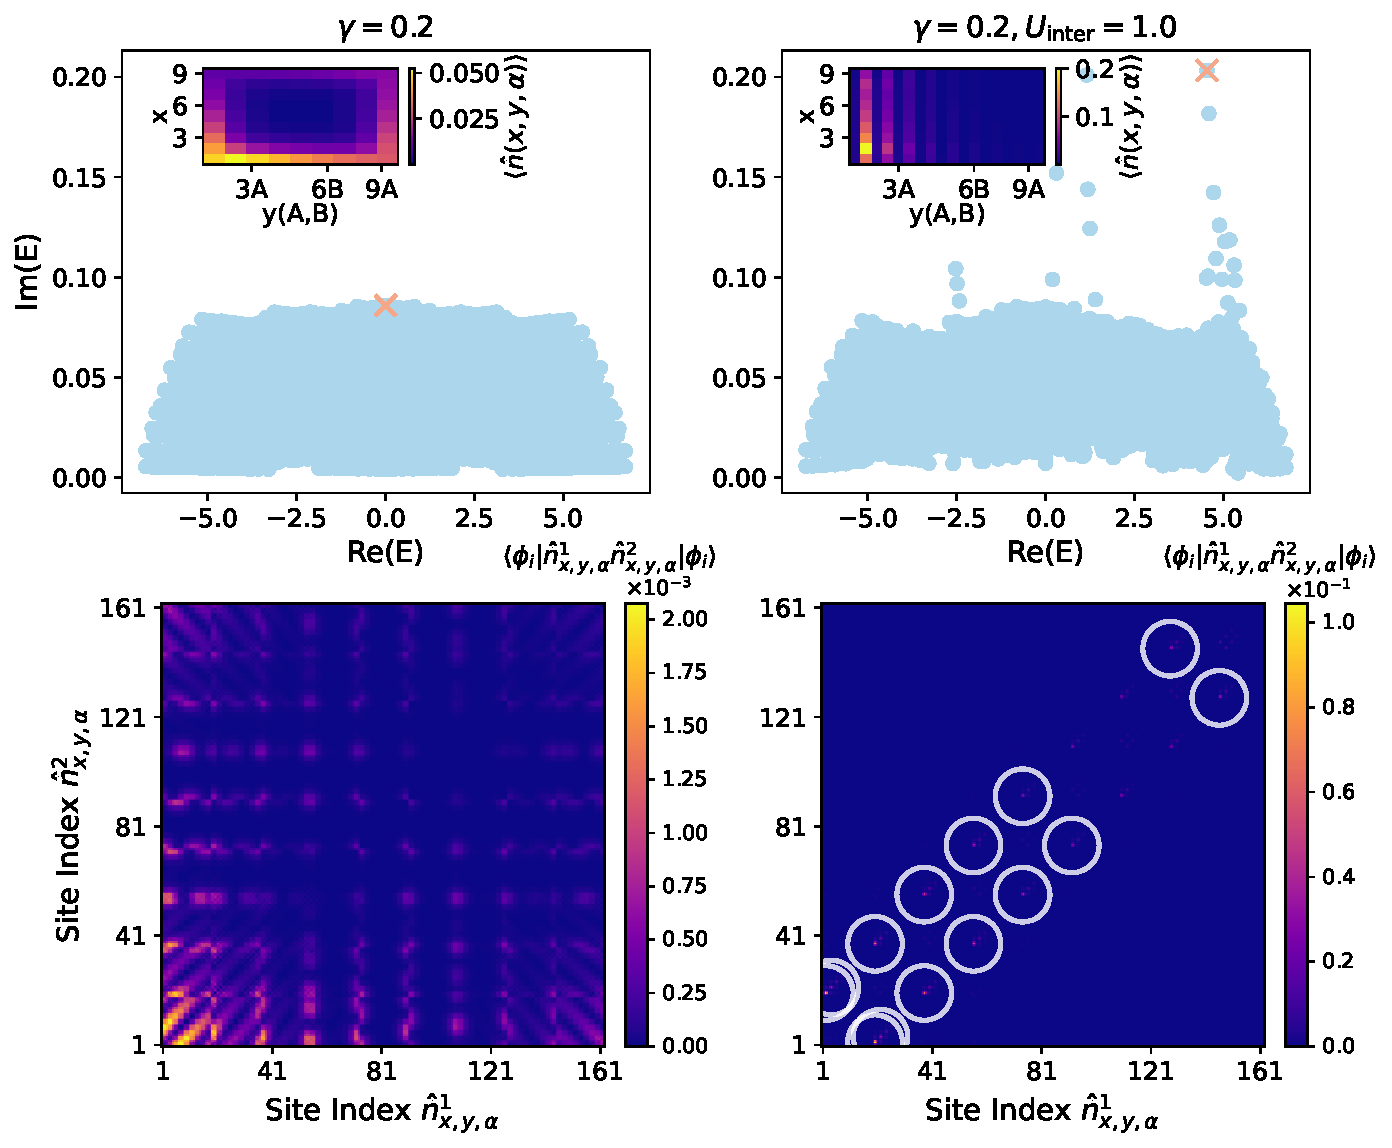
\includegraphics[width=\textwidth]{picture2/Pic_TwoExcitation.pdf}
			% \caption{图片3说明}
			% \label{fig:img3}
		\end{minipage}
		\begin{overpic}[width=0.32\linewidth]{picture2/Mech3.pdf}
			% \put(-98,152){(a1)}
			% \put(-33,152){(a2)}
			% \put(32,152){(a3)}
			% \put(7,54){(c)}
			\put(-118,100){(a)}
			\put(-60,100){(b)}
			\put(-118,52){(c)}
			\put(-60,52){(d)}
			\put(-3,100){(e)}
			% \put(49,54){(d)}
		\end{overpic}
		\caption{
			The spectrum of the non-Hermitian Hamiltonian (a) without interaction and (b) with interaction $\hat{H}_{\text{inter}}$ in the two-excitation subspace. 
			The eigenstate's average particle number $\langle \hat{n}(x,y,\alpha) \rangle$ of the eigenstate with the largest imaginary eigenvalue is shown in the inset. The non-Hermitian gain is applied to the $y=1$ boundary. The energy of eigenstates is indicated by an orange cross in the spectrum. 
			The two-particle correlation function $\langle \phi_i \vert \hat{n}^1 \hat{n}^2 \vert \phi_i \rangle$ between two particles of the eigenstate with the largest imaginary eigenvalue for non-Hermitian Hamiltonians (c) with or (d) without many-body interaction. In (d), the positions where the two-particle correlation function exceeds 0.03 are marked with white circles.
		The system size is $L_x=L_y=9$ and the onsite potential is $u=-1.5$. The non-Hermitian gain is applied to the $y=1$ boundary. 
		(e) Schematic representation of quantum states in the two-excitation subspace with and without $\hat{H}_{\text{inter}}$ many-body interaction. 
		Blue spheres: unit cells; blue downward arrows (red upward arrows): particles at $A$ ($B$) sublattice; black arrows: allowed transitions; blue wavy arrows: non-Hermitian pumping (arrow number indicates strength). 
		The energy splitting induced by many-body interactions is denoted by $U_{\text{inter}}$.}
		\label{fig:02}
	\end{figure*}
	\textit{Hybrid chiral skin correlated states}. We consider the system incorporating the single-particle non-Hermitian Hamiltonian and many-body interactions. 
	A paradigmatic model to show single-particle topological states is the QWZ model~\cite{qi2006topological}. The non-Hermitian part $\hat{H}_{\text{im}}$ is the sum of gain/loss energy on each site, which holds imaginary onsite energy, such as $\hat{H}_{\text{im}} = \sum_{i\in \text{dissi}} \mathrm{i}\tilde{\gamma} \hat{c}_i^{\dagger} \hat{c}_i$ for gain/loss energy, $\hat{c}_{{x}, {y}}^{\dagger}$ ($\hat{c}_{{x}, {y}}$) is the creation (annihilation) operators at site $({x},{y})$.  The system has $L_x$ ($L_y$) unit cells in the x-direction (y-direction) and each unit cell has two sites, labelled as $A$ and $B$. The non-Hermitian term is added along $y=1$ boundary of the system, and this single-particle Hamiltonian reveals chiral skin topology \cite{nakamura2023universal, ma2024non, schindler2023hermitian}.
	%In the following, we focus on the interplay between the non-Hermitian topology and many-body interactions. 
    The additional many-body interaction is
	%\begin{eqnarray}
        \begin{small}
		\begin{align}
			&\hat{H}_{\text{inter}}  = \sum_{{x}=1}^{L_{x}-1} \sum_{{y}=1}^{L_{y}}  U_{\text{inter}} \left(\hat{n}_{{x}, {y}, A}+\hat{n}_{{x}, {y}, B}\right) \left(\hat{n}_{{x}+1, {y}, A}+\hat{n}_{{x}+1, {y}, B}\right)\notag\\
			& + 
			\sum_{{x}=1}^{L_{x}} \sum_{{y}=1}^{L_{y}-1}  U_{\text{inter}} \left(\hat{n}_{{x}, {y}, A}+\hat{n}_{{x}, m_y, B}\right) \left(\hat{n}_{{x}, {y}+1, A}+\hat{n}_{{x}, {y}+1, B}\right), \label{eq:inter_cell}
		\end{align}
        \end{small}
	%\end{eqnarray}
	where $\hat{n}_{{x},{y},\alpha}=\hat{c}_{x,y,\alpha}^{\dagger}\hat{c}_{x,y,\alpha}$ denotes the number operator at $\alpha$ sublattice of the unit cell with position (${x},{y}$). When the many-body interaction above is added, the
	total particle number operator $\hat{N} = \sum_{x,y,\alpha} \hat{n}_{x,y,\alpha}$ still commutes with the total Hamiltonian.
    For the intriguing topological phenomena of non-Hermitian many-body systems~\cite{shen2024enhanced,shimomura2024general,deng2022observing}, their nontrivial topological characteristics exhibit in Fock space and are closely related to particle occupations. These effects motivate our investigation of quantum state distributions across different excitation subspaces and exploration of both the localization behavior and topological properties.

	Considering the commutation between $\hat{N}$ and $\hat{H}$, the dynamics will be confined within the subspace of the same excitation. Since the many-body effect emerges if the excitation is beyond more than one, we concern about the two-excitation subspace, and reveal the interplay between the many-body interactions and non-Hermiticity. 
	In the two-excitation subspace, the spectrum and average particle number at each lattice site of the gain non-Hermitian Hamiltonians 
	%both in the absence and presence of inter-cell interaction $\hat{H}_{\text{inter}}$ 
	are shown in Fig.~\ref{fig:02}.
	Figs.~\ref{fig:02} (a-b) show the energy spectrum
	%, the eigenstate with the largest imaginary eigenvalue, and the average particle number of this eigenstate 
	for the non-Hermitian Hamiltonian without or with the many-body Hamiltonian (Eq.~\ref{eq:inter_cell}). 
    For a non-Hermitian Hamiltonian without interactions, the spectrum exhibits symmetry with respect to the line $\Re(E)=0$ in the complex spectrum plane (Fig.~\ref{fig:02} (a)), consistent with results from single-particle subspaces and previous studies~\cite{nakamura2023universal, ma2024non,schindler2023hermitian}. This symmetry arises because $\hat{H}_{\text{QWZ}}$ and $\hat{H}_{\text{im}}$ possess the anti-$\mathcal{PT}$ symmetry.
	The detailed analysis is provided in Supplementary~\ref{sec:symmetry_Hamiltonian}.
	The inset of the Figs.~\ref{fig:02} (a-b) shows the average particle number at each lattice site for the eigenstate, defined as follows $\langle \hat{n}(x,y,\alpha) \rangle = \langle \phi_i \vert \hat{n}_{x,y,\alpha} \vert \phi_i \rangle$,
	where 
	%$\phi_i$ is eigenstate in two-excitation subspace, 
	$\hat{n}_{x,y,\alpha}$ is number operator at sublattice $\alpha (\alpha=A,B)$ of unit cell $(x,y)$.
	The eigenstate $\vert \phi_i \rangle$ is the eigenstate with the largest imaginary eigenvalue (orange cross in the corresponding Figs.~\ref{fig:02} (a-b)). The eigenstates in the two-excitation subspace are
    \begin{small}
    \begin{equation}
		\begin{split}
			\phi_i =& a_1 \ket{(11)_{1,1}(00)_{1,2}\cdots} + a_2 \ket{(10)_{1,1}(10)_{1,2}\cdots} + \cdots\\
			=& a_1 \hat{c}_{1,1,A}^{\dagger}\hat{c}_{1,1,B}^{\dagger} \ket{0\cdots} + a_2 \hat{c}_{1,1,A}^{\dagger}\hat{c}_{1,2,A}^{\dagger} \ket{0\cdots} + \cdots.
		\end{split}\label{eq2}
	\end{equation}
    \end{small}
	During this work, the notation $\ket{(ab)_{x,y}}$ in Eq.~\ref{eq2} indicates fermion occupation at the unit cell with position $(x,y)$, where $a=1(0)$ denotes the presence (absence) of fermion at $A$ sublattice and $b=1(0)$ denotes the presence (absence) of fermion at $B$ sublattice.
	In the absence of interaction, the multi-particle chiral skin modes can be piled up simply from single-particle chiral skin modes. Consequently, multi-particle states formed by these modes still preserve the characteristic of the chiral skin effect, as shown in the inset of Fig.~\ref{fig:02}(a).
	When many-body interaction $\hat{H}_{\text{inter}}$ is introduced, the results are shown in the Fig.~\ref{fig:02}(b). The many-body interaction $\hat{H}_{\text{inter}}$($U_{\text{inter}}=1.0$) alters eigenvalue distribution and generates more localized eigenstate distribution. 

	The many-body interaction resulting in the super-localization of eigenstates can also be understood from the two-particle correlation function. 
	We show the two-particle correlation function $\langle \phi_i \vert \hat{n}^1_{x,y,\alpha} \hat{n}^2_{x,y,\alpha} \vert \phi_i \rangle$ for the eigenstate with the largest imaginary eigenvalue in Figs.~\ref{fig:02} (c-d). The operator $\hat{n}^1_{x,y,\alpha}$ ($\hat{n}^2_{x,y,\alpha}$) is the number operator of the first (second) particle at the $\alpha$ sublattice of the unit cell $(x,y)$.
	In Fig.~\ref{fig:02}(c), the correlation function is of the order of $10^{-3}$. While with the inter-cell interaction, the two-particle correlation function reveals a strong spatial correlation between the location of two particles. It reaches approximately $10^{-1}$ as shown in Fig.~\ref{fig:02}(d).
    %Locations where the two-particle correlation function exceeds $0.03$ are indicated by white circles in Fig.~\ref{fig:02}(d).
	Particles preferentially occupy adjacent sites ($\Delta x =1$) along $y=1$, and the particles are more localized on sublattice $B$. 
	For this strong correlation emerges in the localized state in Fig.~\ref{fig:02}(d), they are named as \textit{hybrid chiral skin correlated states}, which are much localized compared to the conventional chiral skin modes (Fig.~\ref{fig:02}(c)).
	
	\textit{Mechanism}. The emergence of hybrid chiral skin correlated states arises from a competitive mechanism: the chiral skin effect drives particles to accumulate at the corners of the system, while many-body interactions suppress particle transitions from unit cells with gain ($y=1$) to unit cells without gain ($y \geq 2$) by inducing energy level splitting ($\Delta E \propto U_{\text{inter}}\langle n_i n_j \rangle$), thereby influencing the system's topological properties.
	The above mechanism of generating such hybrid chiral skin correlated states can also be analyzed with the aid of Fock space representation, as illustrated in Fig.~\ref{fig:02}(e). 
	To achieve a more compact presentation of Fig.~\ref{fig:02}(e), unit cells with gain ($\forall x$ and $y$ = 1) are arranged first, followed by those without gain. The consequence in terms of the time evolution is explained as follows:
	\begin{enumerate}
		\item In Fig.~\ref{fig:02}(e), $\ket{\uparrow}$ represents a particle at the higher-energy $B$ sublattice (when $u<0$), while $\ket{\downarrow}$ represents a particle at the $A$ sublattice of the unit cell. 
		Blue spheres represent the unit cells.
		Notably, when both $\ket{\uparrow}$ and $\ket{\downarrow}$ coexist in a unit cell, it indicates both $A$ and $B$ sublattices are occupied.
        %one particle is located at the $A$ sublattice and the other is located at the $B$ sublattice. 
		\item The blue wavy lines denote the non-Hermitian pumping governed by $\hat{H}_{\text{im}}$, which is restricted to the unit cells with subscripts $(\forall x,y=1)$. Under time evolution, because the gain in $\hat{H}_{\text{im}}$ are applied to the unit cells along $y=1$ boundary, the quantum state amplitudes undergo exponential amplification proportional to their occupation number at the unit cells with the position $y=1$ before normalization. For instance, the state $\xi_1 \ket{(01)_{1,1}(01)_{2,1}\cdots(00)_{1,2}\cdots} + \xi_2\ket{(00)_{1,1}(01)_{2,1}\cdots(01)_{1,2}\cdots}$ evolves under time $\mathrm{d}t$ to state $\xi_1 e^{2\gamma \mathrm{d}t} \ket{(01)_{1,1}(01)_{2,1}\cdots(00)_{1,2}\cdots} + \xi_2 e^{\gamma \mathrm{d}t} \ket{(00)_{1,1}(01)_{2,1}\cdots(01)_{1,2}\cdots}$ before normalization, where the exponents reflect the different pumping strengths to coefficients $\xi_1$ and $\xi_2$. 
		\item Black arrows indicate the hopping term in $\hat{H}_{\text{QWZ}}$, and the magnitude of the transition is $1/2$. The vertical axis quantifies the total energy, comprising contributions from both the onsite energy ($u=-1.5$) in $\hat{H}_{\text{QWZ}}$ and the many-body interaction.
	\end{enumerate}

	
	Concerning with the second key point above, the non-Hermitian evolution drives the particles into the specific subspace
	$\mathscr{H}_{\text{gain}}=\left\{ \ket{(01)_{1,1}(01)_{2,1}\cdots(00)_{1,2}\cdots}, \cdots \right\}$,
	where both particles are at the $y=1$ boundary.
	Under the time evolution governed by the non-Hermitian term $e^{-\mathrm{i}\hat{H}_{\text{im}} \mathrm{d}t}$, when both sites occupied by the fermions exhibit gain, these quantum states experience stronger gain. 
	The pumping effeciency into the subspace $\mathscr{H}_{\text{gain}}$ scales with the overlap of quantum states with $\mathscr{H}_{\text{gain}}$. 
	%is proportional to the probability amplitude of each state within this subspace. 

    \begin{figure*}[htbp]
		\begin{minipage}[b]{0.61\textwidth}
			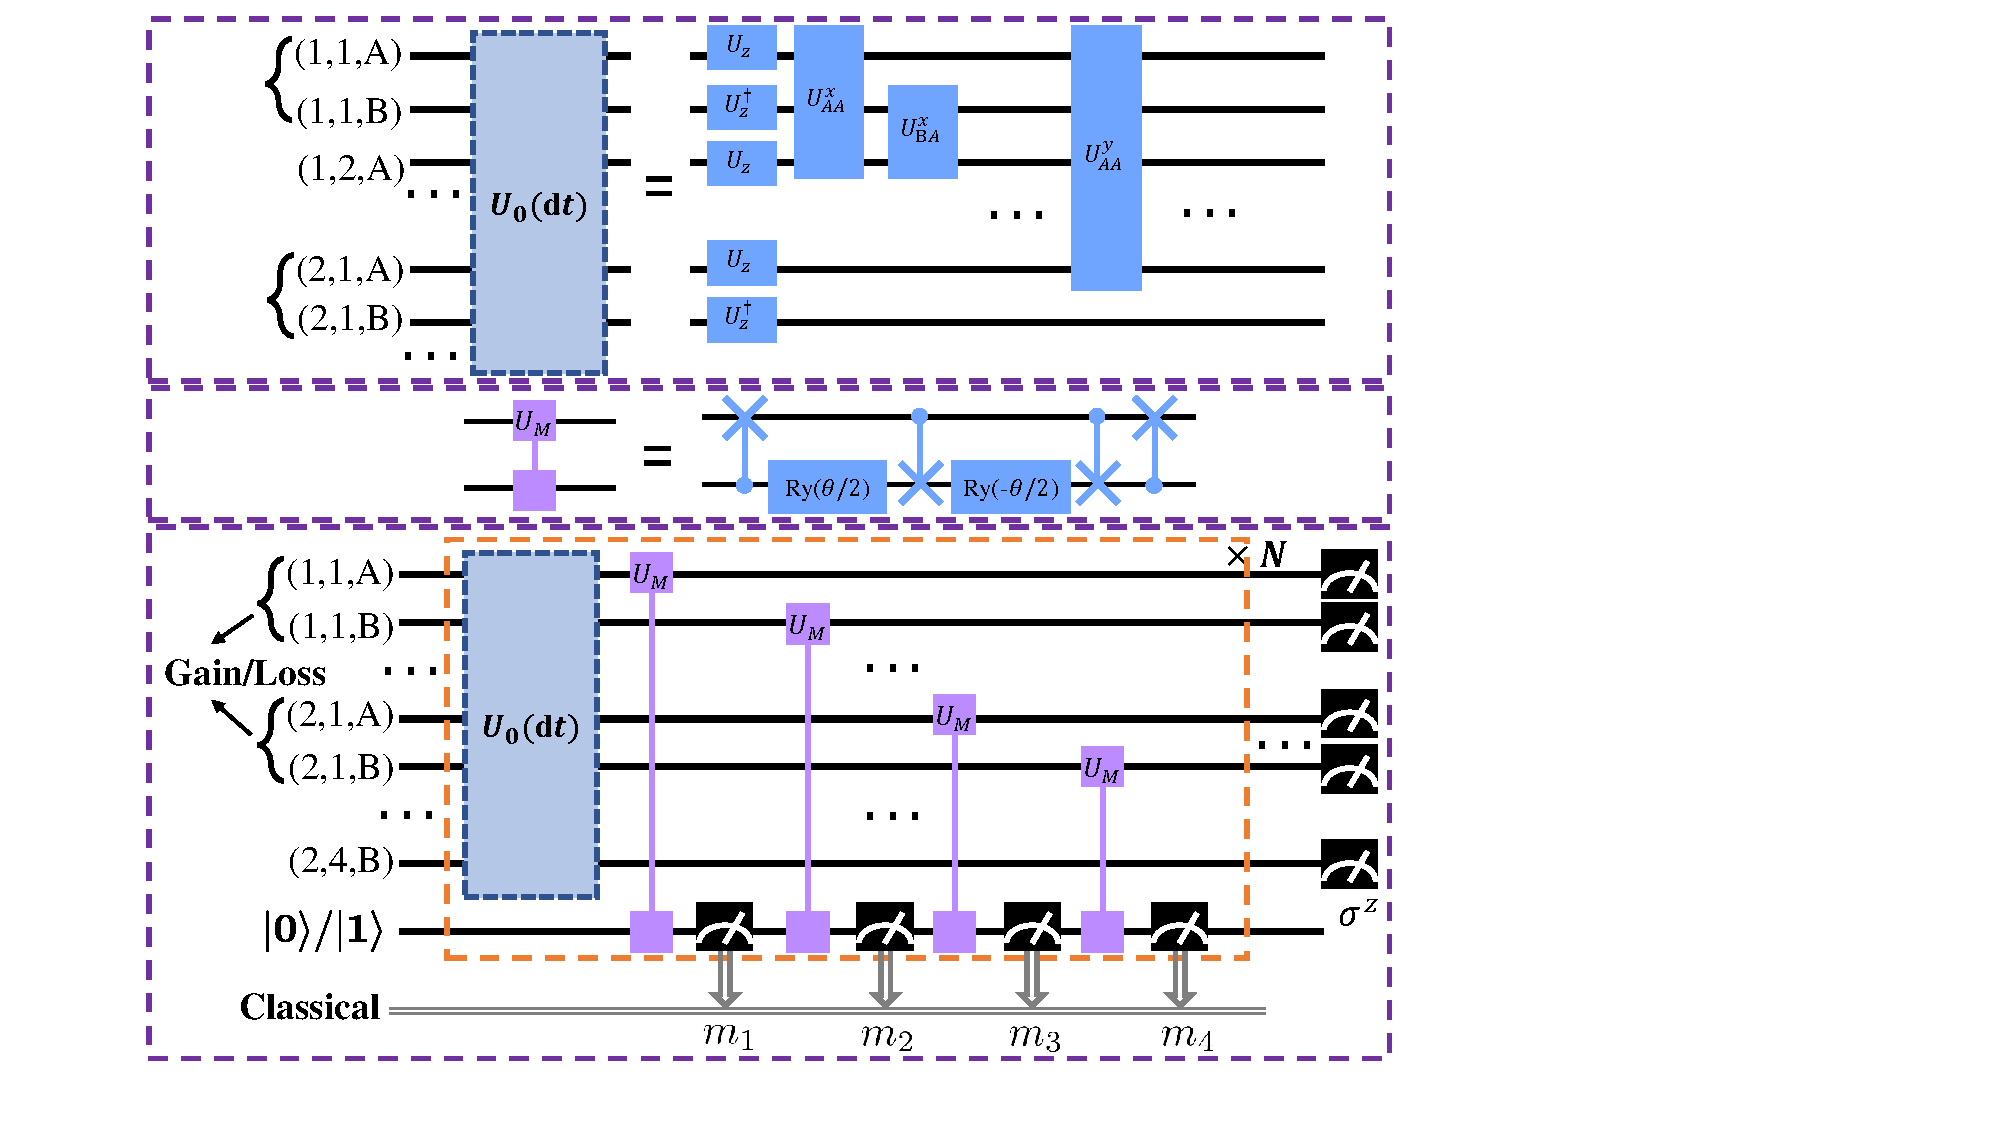
\includegraphics[width=\textwidth]{Picture/RunCircuit.pdf}
			% \caption{图片3说明}
			% \label{fig:img3}
		\end{minipage}
		\hfill
		\begin{minipage}[b]{0.37\textwidth}
			% 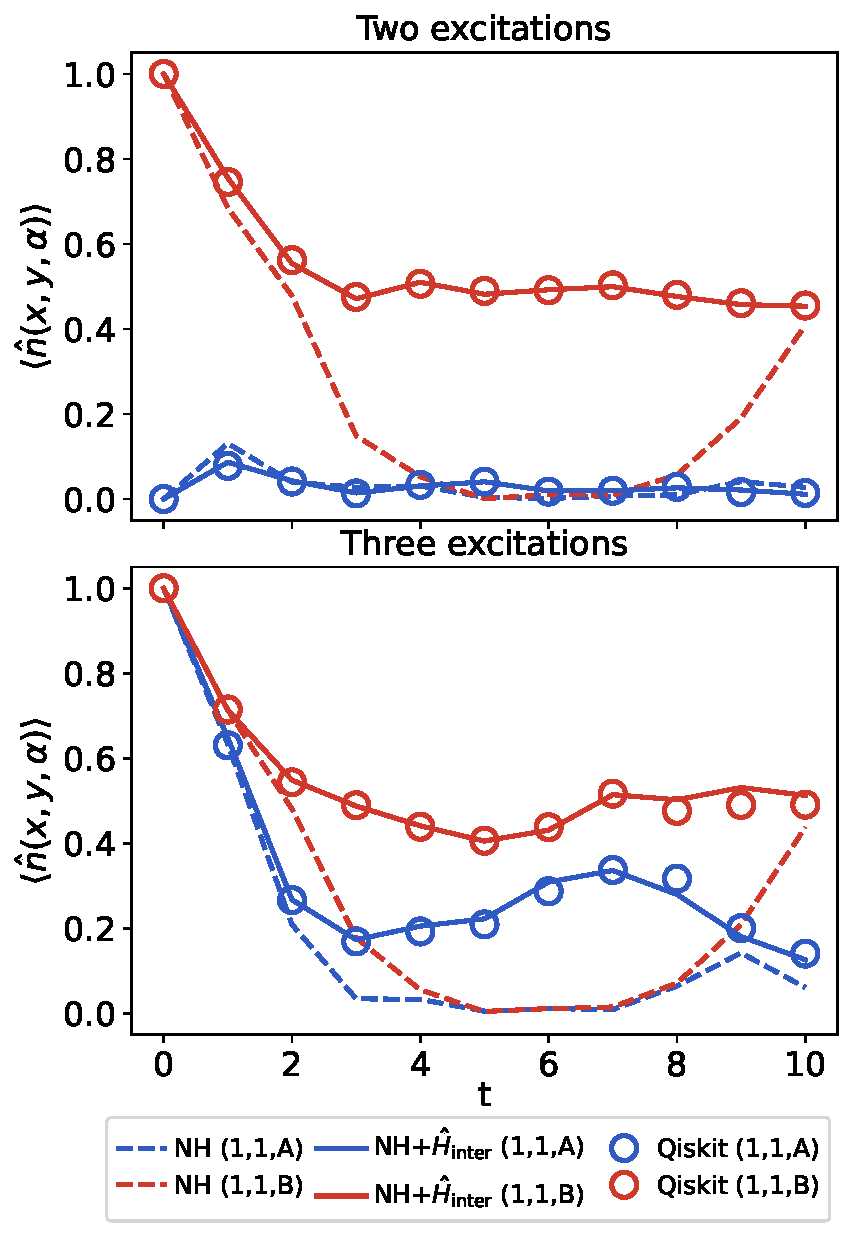
\includegraphics[width=\textwidth]{Picture/MQC_Comp.pdf}
			\begin{overpic}[width=\linewidth]{Picture/MQC_Comp.pdf}
				% \put(-90,198){(a)}
				% \put(7,54){(c)}
				\put(-118,97){(a)}
				\put(1,97){(b)}
				\put(1,55){(c)}
				% \put(49,54){(d)}
			\end{overpic}
			% \caption{图片4说明}
			% \label{fig:img4}
		\end{minipage}
		\caption{
		(a) The MQCs implemented in Qiskit for realizing the gain/loss non-Hermitian many-body Hamiltonians. Each qubit represents a lattice site, where the states $\ket{0}/\ket{1}$ correspond to auxiliary qubits used to implement the non-Hermitian evolution on gain/loss lattice sites (marked as 'gain/loss'). The time evolution of the Hermitian part $U_0(\mathrm{d}t)$ is realized with quantum gates. 
		Generalized measurements $M_i$ are implemented by applying two-qubit gates $U_{\text{M}}$ between gain/loss lattice sites and the auxiliary qubit, followed by a single-qubit $\hat{\sigma}_z$ measurement on the auxiliary qubit.
		The two-qubit gates $U_{\text{M}}$ can be realized with CNOT gates and single-qubit $R_y(\theta/2)$ gates. The parameters of the MQCs are $\mathrm{d}t=0.2$,$N=50$.
		Evolution of the average particle number at different lattice sites over time $t$ under the MQCs in (a) for (b) two excitations and (c) three excitations. 
		%The evolution starts from the initial state where two particles are located on the $B$ sublattice of unit cell $(1,1)$ and $(1,2)$. 
		For two excitations, the initial state consists of two particles located at $(1,1,B)$ and $(2,1,B)$. For three excitations, the initial state consists of three particles located at $(x,y,\alpha)=(1,1,B), (2,1,B), (1,1,A)$.
		The results are obtained through both the MQCs described in (a) and exact calculations. The system size is $L_x=2,L_y=4$. The interaction strength is $U_{\text{inter}}=1.0$ and the non-Hermitian parameter is $\gamma=0.2$. The parameters of the MQCs are $\mathrm{d}t=0.2$,$N=50$.
		}
		\label{fig:04}
	\end{figure*}
    
    If no many-body interaction exists, the energy degeneracy between states inside and outside the Hilbert space $\mathscr{H}_{\text{gain}}$ allows significant particle leakage from this subspace.
	Through continued non-Hermitian evolution, these quantum states ultimately evolve into chiral skin modes.
	In contrast, when the many-body interaction $\hat{H}_{\text{inter}}$ is added, the significant energy gap $\vert U_{\text{inter}} \vert$ between states within $\mathscr{H}_{\text{gain}}$ and outside suppresses transitions out of $\mathscr{H}_{\text{gain}}$, leading to the more localization. 
	The large energy gap from $\hat{H}_{\text{QWZ}}$ suppresses transitions between $\ket{(01)_{1,1}(01)_{2,1}\cdots(00)_{1,2}\cdots}$ and $\ket{(00)_{1,1}(01)_{2,1}\cdots(01)_{1,2}\cdots}$ 
	%Notably, the above gap exceeds the energy gap between $\ket{(10)_{1,1}(10)_{2,1}\cdots(00)_{1,2}\cdots}$ and $\ket{(00)_{1,1}(10)_{2,1}\cdots(10)_{1,2}\cdots}$.
	. So the state $\ket{(01)_{1,1}(01)_{2,1}\cdots(00)_{1,2}\cdots}$ is kept remained during the evolution.
    It is noted that the above hybrid chiral skin correlated states arise from the interplay between non-Hermitian topology and many-body interactions. The localized states induced solely by the interplay between non-Hermiticity and many-body interaction $\hat{H}_{\text{inter}}$ are analyzed in the Supplementary~\ref{sec:NHMBL}.
	This analysis reveals a fundamental distinction between localization mechanisms with or without topological effects.
	%demonstrating that these two localization mechanisms in the presence and absence of topology are fundamentally distinct. 
    The amplitude enhancement and energy gap isolation of $\ket{(01)_{1,1}(01)_{2,1}\cdots(01)_{n,1}(00)_{n+1,1}\cdots(00)_{1,2}\cdots}$ enable the emergence of hybrid chiral skin correlated states in the $n$-excitation subspace. 
	The hybrid chiral skin correlated states can be found in the higher-excitation subspace and the higher-dimensional system. Details have been shown in the End Matter.
    In addition, the hybrid chiral skin correlated states are also shown in different cases, see from Supplementary~\ref{sec:AllP} to \ref{sec:appendicD_loss}.
	
    
	\textit{The demonstration of hybrid correlated topological states with MQCs}.
	The above intriguing phenomena can be uncovered based on MQCs. The corresponding circuit for simulating a non-Hermitian Hamiltonian we adapted in Qiskit is as Fig.~\ref{fig:04} (a). The time evolution of the Hermitian part, including $\hat{H}_{\text{QWZ}}$ and $\hat{H}_{\text{inter}}$, is implemented through quantum gates. 
	%To simulate the dynamics in quantum circuits, we first apply the Jordan-Wigner transition to the Hamiltonian. 
	Qubit state $\ket{1}$ ($\ket{0}$) represents the occupation (unoccupation) of the site. 
	The anticommutation relation of fermionic operators introduces a phase factor -1 when two fermions are exchanged. To maintain this property in our qubit representation, we implement the Jordan-Wigner transformation on the Hamiltonian.
    The time evolution of the hopping term $e^{-\mathrm{i} (\hat{c}_{1,2,A}^{\dagger} \hat{c}_{1,1,A} + \text{h.c.})\mathrm{d} t/2}$ can be transformed into a three-qubit gate via the Jordan-Wigner transformation, represented as $e^{-\mathrm{i} (\hat{\sigma}_{1,2,A}^{\dagger} \hat{\sigma}^z_{1,1,B}\hat{\sigma}_{1,1,A}^{-} + \text{h.c.})\mathrm{d} t/2}$. This three-qubit gate is marked as $U_{AA}^x$ in Fig.\ref{fig:04}. Similarly, the time evolution of other terms in the Hermitian Hamiltonian can be implemented via quantum circuits. For example, $U_{BA}^x$ in Fig.\ref{fig:04} corresponds to the time evolution of the hopping term between sites $(1,1,B)$ and $(1,2,A)$, while $U_{AA}^y$ represents the time evolution of the hopping term between sites $(1,1,A)$ and $(2,1,A)$. The many-body interaction terms can be realized using two-qubit gates.

	For the non-Hermitian part, the corresponding time evolution is implemented through the measurements on one ancillary qubit. 
	All generalized measurements in our scheme can be implemented through only one ancilla. To realize the gain (loss) non-Hermitian Hamiltonian dynamics, we initialize the ancillary qubit to state $\ket{1}$ ($\ket{0}$). And we apply the two-qubit unitary gates $U_M$ to the dissipative sites and the ancillary qubit, as shown in Fig.~\ref{fig:04}. The unitary gates $U_M$ can be realized through CNOT gates and $R_y(\theta) = e^{-\mathrm{i} \hat{\sigma}_y \theta}$ ($\theta = \arccos(e^{-\gamma \mathrm{d}t})$) gates.
	After applying the unitary gates, we measure the ancillary qubit and store the measurement outcomes in classical registers. 
	We postselect quantum trajectories when the results on the classical register are $\ket{1}$($\ket{0}$) to realize the evolution of gain(loss) non-Hermitian Hamiltonians. By repeating this circuit $N$ times, we effectively simulate non-Hermitian dynamics of time $N\mathrm{d}t$. All details have been shown in Supplementary~\ref{sec:scheme_method}.
	%我们选择所有经典寄存器结果都是$\ket{1}$($\ket{0}$)的量子轨迹，可以实现增益(耗散)非厄米哈密顿量的演化。

	The comparisons between the results of the MQC and exact time-evolution are given in Fig.~\ref{fig:04} (b) and (c). 
	We consider a two-dimensional lattice with dimension $L_x=2$ and $L_y=4$, and the gain is implemented on the boundary at $y=1$. 
	There are initially two fermions at lattice sites $(1,1,B)$ and $(2,1,B)$, %Through numerical calculations, 
    and we investigate the system's evolution under both the non-Hermitian without (dashed lines) and with many-body Hamiltonian (solid lines). Additionally, we simulate the evolution with the quantum circuit shown in Fig.~\ref{fig:04} (a) (hollow circles) and measure the average article number $\langle \hat{n}(x,y,\alpha)\rangle$ at subsequent time. The blue (red) curves and points in Fig.~\ref{fig:04} (b) represent the average particle number at site $(1,1,A)$ ($(1,1,B)$).
	The consistencies about the two-excitation (Fig.~\ref{fig:04} (b)) and three-excitation (Fig.~\ref{fig:04} (c)) validate the successful simulations of non-Hermitian many-body Hamiltonian based on MQCs. 
	%At time $t=4$, the results under the non-Hermitian Hamiltonian and the non-Hermitian many-body Hamiltonian show significant differences. 
	For the evolution of the non-Hermitian Hamiltonian, we observe complete population transfer from site $(1,1,B)$ followed by revival.
	% Specifically, under non-Hermitian Hamiltonian, the particle at site $(1,1,B)$ completely jumps to other sites and then returns. 
	In contrast, the non-Hermitian many-body Hamiltonian drives the system toward a steady state with frozen particle number distributions.
	% In contrast, under non-Hermitian many-body Hamiltonian, the system quickly evolves into a steady state, where the particle number at each site remains constant. 
	These measurable occupation patterns provide direct experimental signatures of how many-body interactions fundamentally alter non-Hermitian quantum dynamics.

	\textit{Experimental proposal}. The approach proposed here can be further experimentally demonstrated using superconducting qubits, trapped ions, or photonic quantum processors by engineering non-reciprocal couplings and controlled dissipation. State-of-the-art noisy intermediate-scale quantum (NISQ) devices, featuring hundreds of qubits, provide a viable platform for implementation. For instance, superconducting qubit array with tunable couplings and high coherence \cite{guo2021observation, preskill2018quantum, wu2021strong} or large-scale photonic quantum simulators with programmable linear optical networks \cite{zhong2020quantum, madsen2022quantum, zhu2024dynamically} could be employed to realize the MQC implementation. Linear qubit gates can be readily implemented using parametric couplers for superconducting qubits or directional couplers and phase modulators for photonic systems \cite{zhu2024large}. A key challenge in realizing many-body non-Hermitian dynamics in MQCs is the implementation of controlled gain or loss. Fortunately, a single ancillary qubit suffices to simulate all necessary generalized measurements. In photonic systems, engineered loss can be introduced via additional modes or waveguide couplings~\cite{hoch2025quantum, carolan2020variational}, while superconducting platforms can leverage mid-circuit measurements to emulate non-Hermiticity~\cite{shen2024enhanced,shen2025observation}. After preparing the Hamiltonian evolution on quantum hardware, exponential localization at boundaries can be observed through qubit measurements or photon detection. Therefore, our proposal can be directly implemented in state-of-the-art superconducting and photonic quantum platforms. 
    %Thus, this work paves the way for exploring non-Hermitian topology in NISQ devices.

	\textit{Conclusion}. Applying gain/loss at the boundaries of a system gives rise to single-particle topological phenomena, such as the chiral skin effect. Upon introducing many-body interactions, we uncover hybrid chiral skin correlated states, which are distinct from multi-particle chiral skin modes. This distinction can be revealed through both site-resolved occupation numbers and correlation functions, highlighting the nontrivial interplay between non-Hermitian topology and many-body interaction. 
	To systematically explore non-Hermitian many-body physics, we develop a programmable MQCs framework based on the universality of digital quantum computers. 
	With this MQCs framework, we simulate these hybrid states on Qiskit using only a single ancillary qubit in two-dimensional lattice configurations. 
	Our study of the interplay between non-Hermitian topology and many-body interactions not only establishes a concrete route toward simulating and controlling non-Hermitian many-body phenomena in two-dimensional systems, but also offers broadly applicable insights for future studies of correlated open quantum matter.

    \section*{Acknowledgements}
	We acknowledge the financial support in part by National Natural Science Foundation of China grant No.12374473 and No.12174215, Taishan Scholars Program.

    % Create the reference section using BibTeX:
	\bibliographystyle{apsrev4-1}
	%\bibliographystyle{unsrt}
	\bibliography{reference.bib}

\clearpage

	\section*{End Matter~\label{sec:method}}
	\subsection{Three-excitation Subspace~\label{sec:three_excitation}}

	So far, we have focused on the two-excitation subspace. In fact, the interplay between topological states and many-body interactions persists even in the higher-excitation subspace. The hybrid chiral skin correlated states can also be found. 
	We consider a two-dimensional lattice with size $L_x = L_y = 5$ for our investigation. For computational convenience, we focus on the three-particle excitation subspace due to the commutation of the particle number operator and Hamiltonian. 
	Fig.~\ref{fig:03a} (a) show the energy spectrum
	%, the eigenstate with the largest imaginary eigenvalue, and the average particle number of this eigenstate 
	for the non-Hermitian Hamiltonian with many-body interactions. 
	The spectrum of the non-Hermitian Hamiltonian does not exhibit symmetry with respect to the imaginary axis due to anti-$\mathcal{PT}$ symmetry in the presence of many-body interactions. 
	The basis in the three-excitation subspace are
	% $\{\ket{11100\cdots}, \ket{11010\cdots}, \ket{10110\cdots},\cdots\}$, 
	\begin{equation}
		\begin{split}
		\{\ket{(11)_{1,1}(10)_{1,2}(00)_{1,3}\cdots}, \ket{(11)_{1,1}(01)_{1,2}(00)_{1,3}\cdots}, \\
		\ket{(10)_{1,1}(11)_{1,2}(00)_{1,3}\cdots},\cdots\}, 
		\end{split}
	\end{equation}
	which represent all possible configurations of three fermions in the system. 
	The eigenstates in the three-excitation subspace are expressed as 
	\begin{equation}
		\begin{split}
			\phi_i^3 =& a_1 \ket{(11)_{1,1}(10)_{1,2}(00)_{1,3}\cdots} +\\
			&a_2 \ket{(11)_{1,1}(01)_{1,2}(00)_{1,3}\cdots} +\\
			&a_3 \ket{(10)_{1,1}(11)_{1,2}(00)_{1,3}\cdots} + \cdots\\
			=& a_1 \hat{c}_{1,1,A}^{\dagger}\hat{c}_{1,1,B}^{\dagger}\hat{c}_{1,2,A}^{\dagger} \ket{0\cdots} +\\
			&a_2 \hat{c}_{1,1,A}^{\dagger}\hat{c}_{1,1,B}^{\dagger}\hat{c}_{1,2,B}^{\dagger} \ket{0\cdots} + \\
			&a_3 \hat{c}_{1,1,A}^{\dagger}\hat{c}_{1,2,A}^{\dagger}\hat{c}_{1,2,B}^{\dagger} \ket{0\cdots} + \cdots.
		\end{split}
	\end{equation}
	%The horizontal axis represents different basis, and each basis corresponds to a three-particle quantum state, as shown in the inset of Fig.\ref{fig:03}(a). 
	Fig.~\ref{fig:03a} (a) show the average particle number at each lattice site for the eigenstate. 
	%Note that the eigenstates of the non-Hermitian Hamiltonian in Fig.~\ref{fig:03} (b3) is not clear, because the calculation is restriction to system size $L_x=L_y=5$.
	Consistent with the above analyses in the two-excitation subspace, the introduction of many-body interactions leads to localization phenomena in both the eigenstates and the average particle number.

	\begin{figure}[h]
		\centering
		\begin{overpic}[width=1.0\linewidth]{picture2/ThreeExcitation_data.pdf}
			\put(5,40){(a)}
			\put(47,40){(b)}
		\end{overpic}
		\caption{
		(a) The spectrum and eigenstate's average particle number $\langle \hat{n}(x,y,\alpha) \rangle$ of non-Hermitian Hamiltonian with interaction $\hat{H}_{\text{inter}}$ in the three-excitation subspace. 
		The complex energy of eigenstate is marked by an orange cross in the spectrum. 
		(b) The three-particle correlation function $\langle \phi_i \vert \hat{n}^1_{x,y,\alpha} \hat{n}^2_{x,y,\alpha} \hat{n}^3_{x,y,\alpha} \vert \phi_i \rangle$ bwteen three particles of the eigenstate with the largest imaginary eigenvalue of non-Hermitian Hamiltonians with interaction $\hat{H}_{\text{inter}}$. The system size is $L_x=L_y=5$ and the onsite potential is $u=-1.5$. The non-Hermitian gain is applied to the $y=1$ boundary.
		}
		\label{fig:03a}
	\end{figure} %label from y=1 and x=1?

	We show the three-particle correlation function $\langle \phi_i \vert \hat{n}^1_{x,y,\alpha} \hat{n}^2_{x,y,\alpha} \hat{n}^3_{x,y,\alpha} \vert \phi_i \rangle$ for the eigenstate with the largest imaginary eigenvalue in Fig.~\ref{fig:03a} (b). 
	For the inter-cell interaction case, the three-particle correlation function reveals strong spatial correlation between the locations of three particles. Particles preferentially occupy adjacent sites ($\Delta x =1$) along $y=1$. The particles are also more localized on sublattice $B$. The details are shown in Supplementary~\ref{sec:three_excitation}.


	Here, we have discussed the hybrid chiral skin correlated states in the two and three-excitation subspaces. The many-body interaction induces these strong localized states, which cannot be found in the single-particle non-Hermitian Hamiltonian. This hybrid state can exist in the even more excitation subspaces, and the mechanism is similar as those in two and three-excitation subspace. 
	When the gain is applied at $y=1$ boundary, the amplitude of state $\ket{(01)_{1,1}(01)_{2,1}\cdots(01)_{n,1}(00)_{n+1,1}\cdots(00)_{1,2}\cdots}$ is enhanced compared to other states in which particles occupy unit cells without gain ($y\neq 1$), under the evolution of $\hat{H}_{\text{im}}$. Moreover, this state is isolated from lower-energy states by a large gap under the evolution of the Hermitian Hamiltonians, such as $\hat{H}_{\text{QWZ}}$ and $\hat{H}_{\text{inter}}$, while other states are either degenerate or separated by relatively small gaps. The amplitude enhancement and energy gap isolation of $\ket{(01)_{1,1}(01)_{2,1}\cdots(01)_{n,1}(00)_{n+1,1}\cdots(00)_{1,2}\cdots}$ enable the emergence of hybrid chiral skin correlated states in the $n$-excitation subspace. 


	\subsection{3D system~\label{sec:appendC_3D}}

	\begin{figure}[h]
		\centering
		\begin{overpic}[width=1.0\linewidth]{Picture/SI/SI_3DCSTISpetrum2.pdf}
			\put(4,97){(a1)}
			\put(44,97){(b1)}
			% \put(7,54){(c)}
			\put(4,61){(a2)}
			\put(44,61){(b2)}
			\put(4,24){(a3)}
			\put(44,24){(b3)}
		\end{overpic}
		%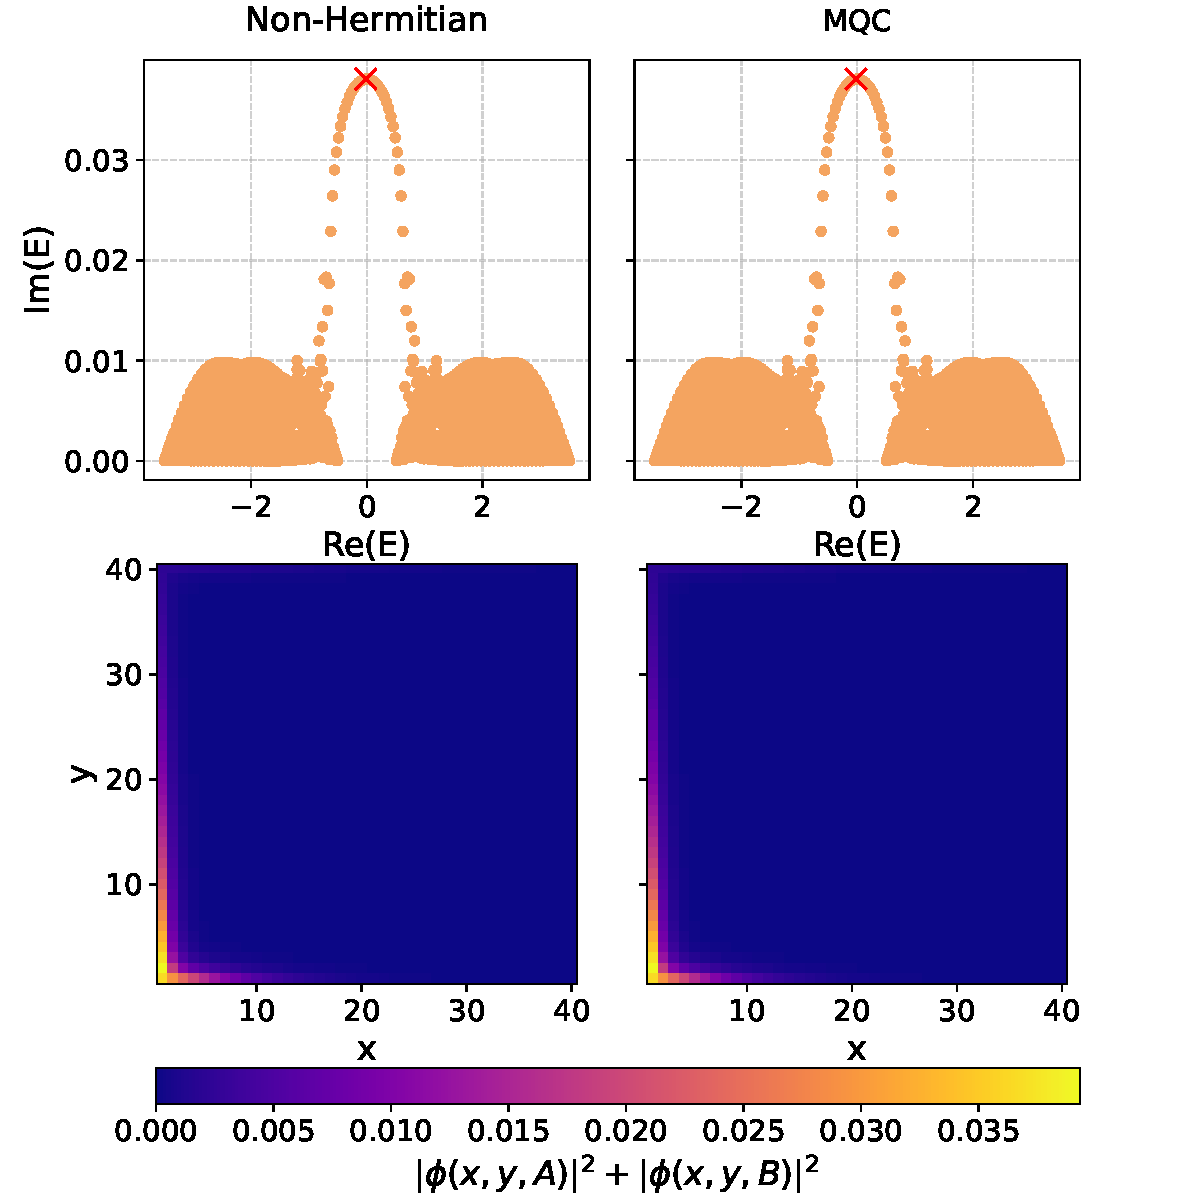
\includegraphics[width=1.\linewidth]{Picture/SingleExcitation_Comp.pdf}
		\caption{
		In the two-excitation subspace, the comparison of the spectrum and eigenstates between the non-Hermitian Hamiltonian with or without $\hat{H}_{\text{inter}}$ many-body interaction. The Hermitian part is the three-dimensional chiral symmetric topological insulator. The non-Hermitian gain ($\gamma=0.2$) is applied on unit cells at the $z=1$ boundary.
		(a1) The spectrum of a non-Hermitian Hamiltonian without interaction.
		(b1) The spectrum of a non-Hermitian Hamiltonian with interaction.
		(a2) The probability distribution of the eigenstates of a non-Hermitian Hamiltonian without interaction. 
		(b2) The probability distribution of the eigenstates of a non-Hermitian Hamiltonian with interaction.
		(a3) The average particle number per lattice site for the eigenstate in (a2).
		(b3) The average particle number per lattice site for the eigenstate in (b2).
		The system size is $L_x=L_y=3,L_z=6$.
		}
		% \label{fig:13}
		\label{fig:16}
	\end{figure} %label from y=1 and x=1?
	We consider the three-dimensional chiral symmetric topological insulator as an example to study the hybrid chiral skin correlated states in higher dimensions. The Hamiltonian of the 3D chiral symmetric topological insulator in real-space is
	\begin{equation}
		\begin{split}
			\hat{H}_{\text{CSTI}} = \sum_{x,y,z} \hat{c}_{x,y,z}^{\dagger}\hat{c}_{x,y,z} \otimes (\hat{\sigma}_x \hat{\tau}_x - 2 \hat{\sigma}_0 \hat{\tau}_y) + \\
			\sum_{x,y,z} \hat{c}_{x,y,z+1}^{\dagger}\hat{c}_{x,y,z} \otimes ( \frac{\mathrm{i} \hat{\sigma}_z \hat{\tau}_x}{2} + \frac{\hat{\sigma}_0 \hat{\tau}_y}{2}) + \\
			\sum_{x,y,z} \hat{c}_{x,y+1,z}^{\dagger}\hat{c}_{x,y,z} \otimes (-\frac{\hat{\sigma}_x \hat{\tau}_x}{2} + \frac{\mathrm{i} \hat{\sigma}_y \hat{\tau}_x}{2} + \frac{\hat{\sigma}_0 \hat{\tau}_y}{2})\\
			\sum_{x,y,z} \hat{c}_{x+1,y,z}^{\dagger}\hat{c}_{x,y,z} \otimes ( \frac{\mathrm{i}\hat{\sigma}_x \hat{\tau}_x}{2} + \frac{\hat{\sigma}_0 \hat{\tau}_y}{2} )
		\end{split} % 所有的i其实应该在分母上面，原来的代码在分子下面是不是不对？
	\end{equation}
	where $\sigma_{x,y,z}$ and $\tau_{x,y,z}$ are the Pauli matrices, and $\sigma_0$ is the $2\times 2$ identity matrix. The gain are applied on the $z=1$ boundary of the system. Each unit cell has four sublattices, labeled as $A$, $B$, $C$ and $D$. 
	Figs.~\ref{fig:16} (a1) and (b1) show the spectrum for gain three-dimensional non-Hermitian Hamiltonian with or without many-body interaction. 
	In Fig.~\ref{fig:16} (a2) and (b2), the probability distributions of the eigenstate with the smallest imaginary eigenvalue (orange cross in Figs.~\ref{fig:16} (a1) and (b1)) is shown.
	 Figs.~\ref{fig:16} (a3) and (b3) show the average particle number at each lattice site for the eigenstate.
	The results indicate that the eigenstate of the non-Hermitian many-body Hamiltonian with the largest imaginary eigenvalue is more localized than the eigenstate in the absence of many-body interaction.
	The average particle number at each lattice site reveals that particles predominantly localize at the sites of $x=1$ and $x=3$.
	%$(x,y,z,\alpha)=(1,2,1,B),(1,2,1,C),(3,2,1,B),(3,2,1,C)$. 
	When many-body interactions are introduced, the average particle number of the eigenstate with the largest imaginary eigenvalue concentrates primarily at $(x,y,z,\alpha)=(3,2,1,B),(3,2,1,C)$. This indicates a strong enhancement of spatial localization induced by many-body interactions. 
	%对本征态各个格点的粒子数算符的均值计算表明，粒子数跟多的局域化在格点$(x,y,z,\alpha)=(1,2,1,B),(1,2,1,C),(3,2,1,B),(3,2,1,C)$. 然后非厄米多体哈密顿量的最大虚本征值的本征态则更加局域，它局域在$(x,y,z,\alpha)=(3,2,1,B),(3,2,1,B)$处。


	The introduction of many-body interaction results in the super-localization of eigenstates in the two-excitation subspace, and it is evident by the two-particle correlation function. 
	Here, we show the two-particle correlation function $\langle \phi_i \vert \hat{n}^1_{x,y,z,\alpha} \hat{n}^2_{x,y,z,\alpha} \vert \phi_i \rangle$ for the eigenstate with the largest imaginary eigenvalue in 3D systems (Fig.~\ref{fig:16}). The operator $\hat{n}^1_{x,y,z,\alpha}$ ($\hat{n}^2_{x,y,z,\alpha}$) is the number operator of the first (second) particle at the $\alpha$ sublattice of the unit cell $(x,y,z)$.
	% The correlation patterns remain qualitatively similar between the non-interacting case and intra-cell interaction case. 
	% The results show that the two-particle correlation function in the absence of interaction and in the presence of interaction $\hat{H}_{\text{intra}}$ is similar.  
	In Fig.~\ref{fig:16_supp} (a), the correlation function for non-Hermitian Hamiltonian without inter-cell many-body interaction is of the order of $10^{-3}$. In contrast, for the inter-cell interaction case, the two-particle correlation function reveals strong spatial correlation between the location of two particles. It reaches approximately $10^{-2}$, which approximates the values obtained in the 2D system (Fig.~\ref{fig:02} (b)).
	% Locations where the two-particle correlation function exceeds $0.03$ are indicated by white circles in Fig.~\ref{fig:02}(d).
	Particles preferentially occupy adjacent sites ($\Delta y =1$) at $z=1$ plane, and the particles are more localized on sublattices $B$ and $C$. 
	The localized state in Fig.~\ref{fig:16_supp} (b) are hybrid chiral skin correlated states in a 3D system, which are much localized compared to the conventional chiral skin modes in a 3D system.
	\begin{figure}[h]
		\centering
		\begin{overpic}[width=1.0\linewidth]{picture2/3D_correlation.pdf}
			\put(5,40){(a)}
			\put(51,40){(b)}
		\end{overpic}
		%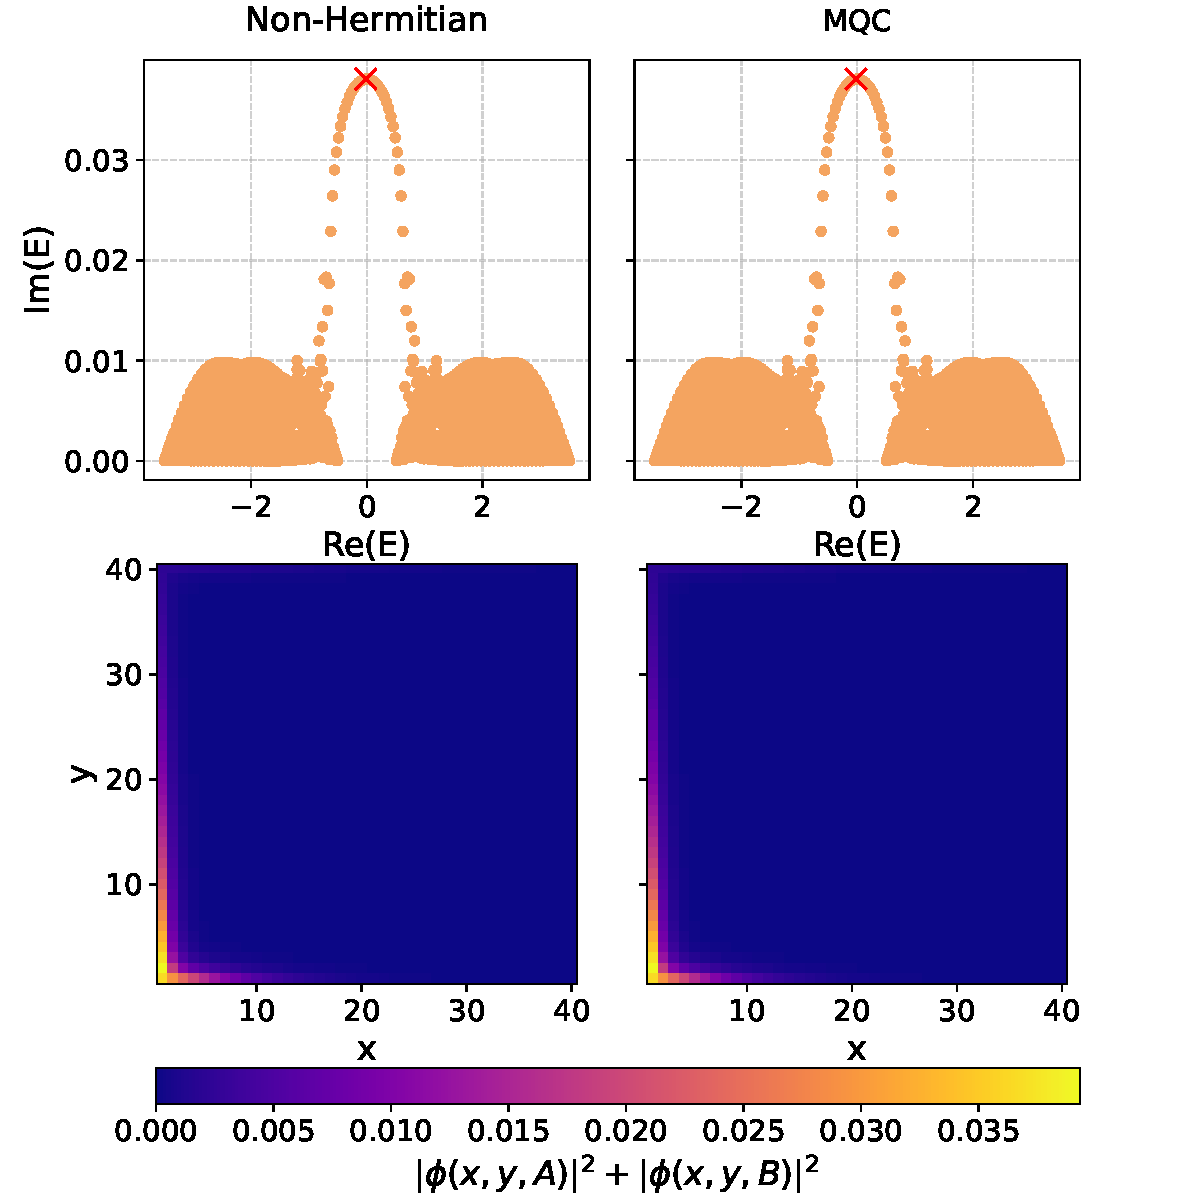
\includegraphics[width=1.\linewidth]{Picture/SingleExcitation_Comp.pdf}
		\caption{In 3D systems, the two-particle correlation function $\langle \phi_i \vert \hat{n}^1 \hat{n}^2 \vert \phi_i \rangle$ between two particles of the eigenstate with the largest imaginary eigenvalue for non-Hermitian Hamiltonians (a) with or (b) without many-body interaction. 
		The system size is $L_x=L_y=3,L_z=6$. The non-Hermitian gain is applied to the $z=1$ boundary.
		}
		% \label{fig:13}
		\label{fig:16_supp}
	\end{figure} %label from y=1 and x=1?

	

	\newpage
	\appendix

	\setcounter{section}{0}

    \section*{Supplementary Materials for "Hybrid chiral skin correlated states in monitored quantum circuits"}
    %\begin{abstract}        
    %\end{abstract}
    %\maketitle
    \setcounter{equation}{0}  % 重置公式计数器为0
    \setcounter{figure}{0}  % 重置公式计数器为0
    \renewcommand{\theequation}{S\arabic{equation}}  % 将公式编号改为S1, S2, S3.
    \renewcommand{\thefigure}{S\arabic{figure}}  % 将公式编号改为S1, S2, S3.
    \renewcommand{\thesubsection}{S\arabic{subsection}}  % 将公式编号改为S1, S2, S3.


	% \section{Non-Hermitian Many-Body Localization: Robustness, Existence Beyond Edge States\label{sec:NHMBL}}
	\subsection{Symmetry of Hamiltonian~\label{sec:symmetry_Hamiltonian}}
	% parity 的变换是交换Ａ，Ｂ两个子晶格。时间反演是共轭。
	The paradigmatic Hamiltonian $\hat{H}_{\text{QWZ}}$ changes sign under a combination of parity and time-reversal transformation, and this symmetry is called anti-$\mathcal{PT}$ symmetry.
	On the other hand, the non-Hermitian Hamiltonian $\hat{H}_{\text{im}}$ remains invariant under parity transformation but changes sign under time-reversal transformation, thus also exhibiting anti-$\mathcal{PT}$ symmetry
	\begin{equation}
		\begin{split}
			\mathcal{PT} \hat{H}_{\text{QWZ}} (\mathcal{PT})^{-1} &= -\hat{H}_{\text{QWZ}} \\
			\mathcal{PT} \hat{H}_{\text{im}} (\mathcal{PT})^{-1} &= -\hat{H}_{\text{im}}.
		\end{split}
	\end{equation}
	However, the interaction Hamiltonian $\hat{H}_{\text{inter}}$ are invariant under a combination of parity ($\mathcal{P}$) and time-reversal ($\mathcal{T}$) operations
	\begin{equation}
		\begin{split}
			\mathcal{PT} \hat{H}_{\text{inter}} (\mathcal{PT})^{-1} = \hat{H}_{\text{inter}}% \\
			% \mathcal{PT} \hat{H}_{\text{intra}} (\mathcal{PT})^{-1} = \hat{H}_{\text{intra}}.
		\end{split}
	\end{equation}
	For systems with anti-$\mathcal{PT}$ symmetry, the energy spectrum is symmetric with respect to the line $\Re(E)=0$ in the complex energy plane, because
	\begin{equation}
		\begin{split}
			\hat{H} \vert \phi \rangle &= E \vert \phi \rangle\\
			\mathcal{PT} \hat{H} (\mathcal{PT})^{-1} \vert \phi \rangle &= - E \vert \phi \rangle\\
			\hat{H} (\mathcal{PT})^{-1} \vert \phi \rangle &= - E^* (\mathcal{PT})^{-1} \vert \phi \rangle.
		\end{split}
	\end{equation}
	This demonstrates that for a system with anti-$\mathcal{PT}$ symmetry, if $\ket{\phi}$ is an eigenstate with energy $E$, there exists another eigenstate $(\mathcal{PT})^{-1} \ket{\phi}$ with energy $-E^*$. Consequently, the energy spectrum of the system is symmetric with respect to the line $\Re(E)=0$ in the energy plane.
	Furthermore, under the $\mathcal{PT}$ transformation, the Hamiltonian $\hat{H}_{\text{inter}}$ with interaction strength $U_{\text{inter}}$ transforms into the Hamiltonian $\hat{H}_{\text{inter}}$ with interaction strength $-U_{\text{inter}}$. Consequently, the energy spectrum and eigenstates of the many-body Hamiltonian with interaction strength $U_{\text{inter}}$ demonstrate a symmetric relationship with those of the Hamiltonian with interaction strength $-U_{\text{inter}}$
	\begin{equation}
		\begin{split}
			\mathcal{PT} (\hat{H}_{\text{QWZ}}+\hat{H}_{\text{inter}}\vert_{U_{\text{inter}}}+\hat{H}_{\text{im}}) (\mathcal{PT})^{-1}\\
			= -(\hat{H}_{\text{QWZ}}+\hat{H}_{\text{inter}}\vert_{-U_{\text{inter}}}+\hat{H}_{\text{im}}).
		\end{split}
	\end{equation}
	The eigenvalues and eigenstates of the Hamiltonians with interaction strength $U_{\text{inter}}$ are denoted as $\{E_{\text{inter}}\}$ and $\{\phi_{\text{inter}}\}$, respectively. For the Hamiltonians with interaction strength $-U_{\text{inter}}$, the eigenvalues and eigenstates are $\{-E_{\text{inter}}^*\}$ and $\{(\mathcal{PT})\phi_{\text{inter}}\}$, respectively.
	
	There is a symmetry between the gain non-Hermitian Hamiltonians and the loss non-Hermitian Hamiltonians. Specifically, we consider a reflection transformation $\mathcal{M}_x$ along the $x$-direction, which maps the unit cells from location $x = 1$ to localization $x = L_x$, and leaves the $y$-coordinate unchanged. In the QWZ model with many-body interactions, there is a symmetry relation under this transformation:
	\begin{equation}
		\begin{split}
			(\mathcal{M}_x \mathcal{K})(\hat{H}_{\text{QWZ}} + \hat{H}_{\text{inter}} + \sum_{i\in \text{dissi}} \mathrm{i}\tilde{\gamma} \hat{c}_i^{\dagger} \hat{c}_i ) (\mathcal{M}_x \mathcal{K})^{-1} \\
			= (\hat{H}_{\text{QWZ}} + \hat{H}_{\text{inter}} - \sum_{i\in \text{dissi}} \mathrm{i}\tilde{\gamma} \hat{c}_i^{\dagger} \hat{c}_i),
		\end{split}
	\end{equation}
	where $\mathcal{K}$ denotes complex conjugation. 
	The eigenvalues and eigenstates of the gain non-Hermitian many-body Hamiltonians are denoted as $\{E_{\text{inter}}\}$ and $\{\phi_{\text{inter}}\}$, respectively. For the loss non-Hermitian many-body Hamiltonians, the eigenvalues and eigenstates are $\{E_{\text{inter}}^*\}$ and $\{(\mathcal{M}_x\mathcal{K})\phi_{\text{inter}}\}$, respectively. 
	According to this symmetry, the chiral skin mode localized at unit cell $(1,1)$ for gain non-Hermitian Hamiltonians, and localized at unit cell $(L_x,1)$ for loss non-Hermitian Hamiltonians.
	This symmetry indicates that the chiral skin mode localizes at unit cell $(1,1)$ for gain non-Hermitian Hamiltonians, and at $(L_x,1)$ for loss non-Hermitian Hamiltonians.


	\subsection{Non-Hermitian Many-Body induced localized states\label{sec:NHMBL}}

	The hybrid chiral skin correlated states emerge from the interplay between the non-Hermitian topology and many-body interactions. To show the novel role of the non-Hermitian topology in the formation of such states, we introduce many-body interactions to the non-Hermitian system without chiral skin modes.
	We demonstrate that non-Hermitian many-body induced localized states appear even in the absence of non-Hermitian topology. However, these states are fundamentally different from the hybrid chiral skin correlated states.
    We show the two-particle correlation function $\langle \phi_i \vert \hat{n}^1_{x,y,\alpha} \hat{n}^2_{x,y,\alpha} \vert \phi_i \rangle$ for the eigenstate with the largest imaginary eigenvalue in Figs.~\ref{fig:02} (c-d).

	\subsubsection{The comparison between the hybrid chiral skin correlated states and non-Hermitian many-body localized states~\label{sec:appendixE_comp}}
    
	\begin{figure*}
		\centering
		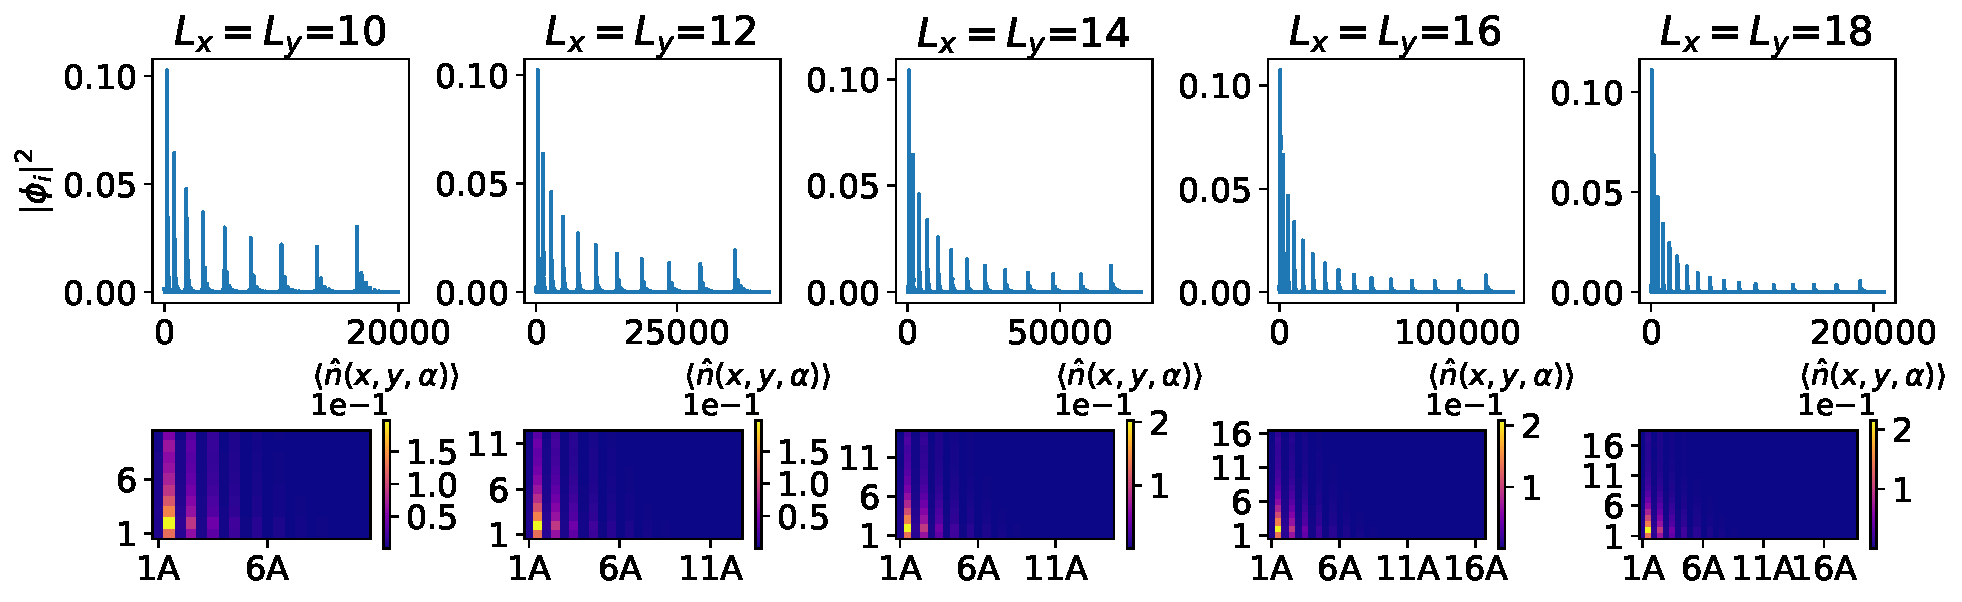
\includegraphics[width=1.\linewidth]{Picture/SI/LargeTwoExcitation.pdf}
		\begin{overpic}[width=1.0\linewidth]{Picture/SI/LargeTwoExcitation_NotTopo.pdf}
			\put(3,61){(a)}
			\put(3,30){(b)}
		\end{overpic}
		\caption{
		The probability distribution of eigenstates with the largest imaginary eigenvalue and average particle numbers $\langle \hat{n}(x,y,\alpha) \rangle$ of the eigenstate per lattice site for different system sizes.
		(a) hybrid chiral skin correlated states, calculated with the Arnoldi method, for system sizes $L_x=L_y=[10,12,14,16,18]$. The onsite potential of the QWZ model is $u=-1.5$, and the QWZ model is a topological insulator.
		(b) Non-Hermitian many-body induced localized states, calculated with the Arnoldi method, for system sizes $L_x=L_y=[10,12,14,16,18]$. 
		The onsite potential of the QWZ model is $u=-2.1$, and the QWZ model is topologically trivial.
		}
		\label{fig:14}
	\end{figure*}
	\begin{figure}[h]
		\centering
		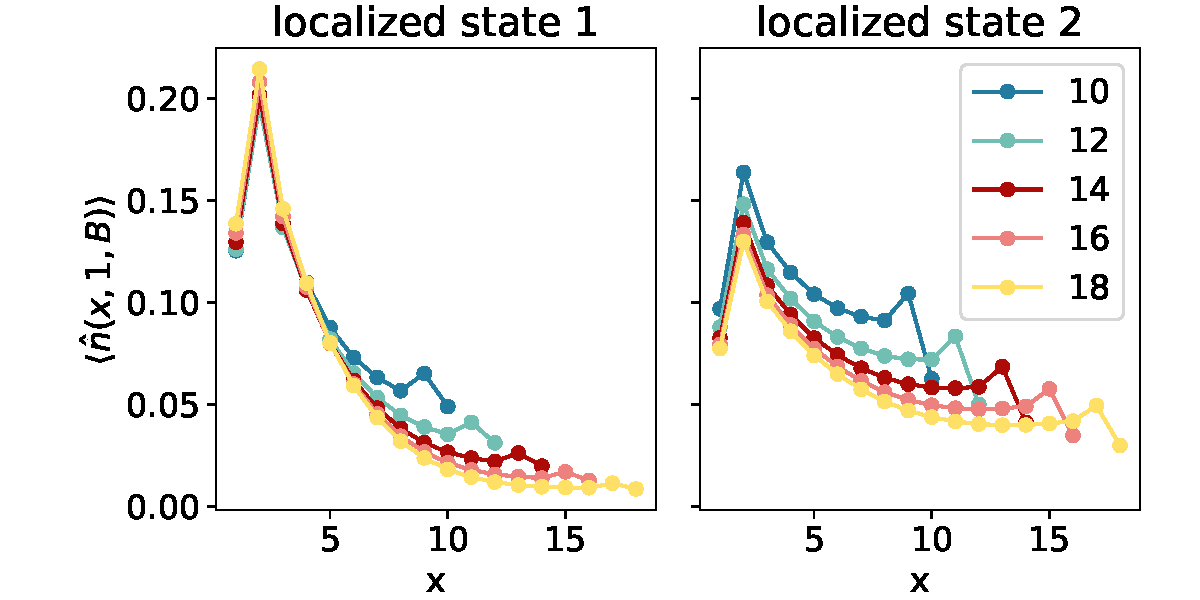
\includegraphics[width=1.\linewidth]{Picture/SI/SI_Comp1.pdf}
		% 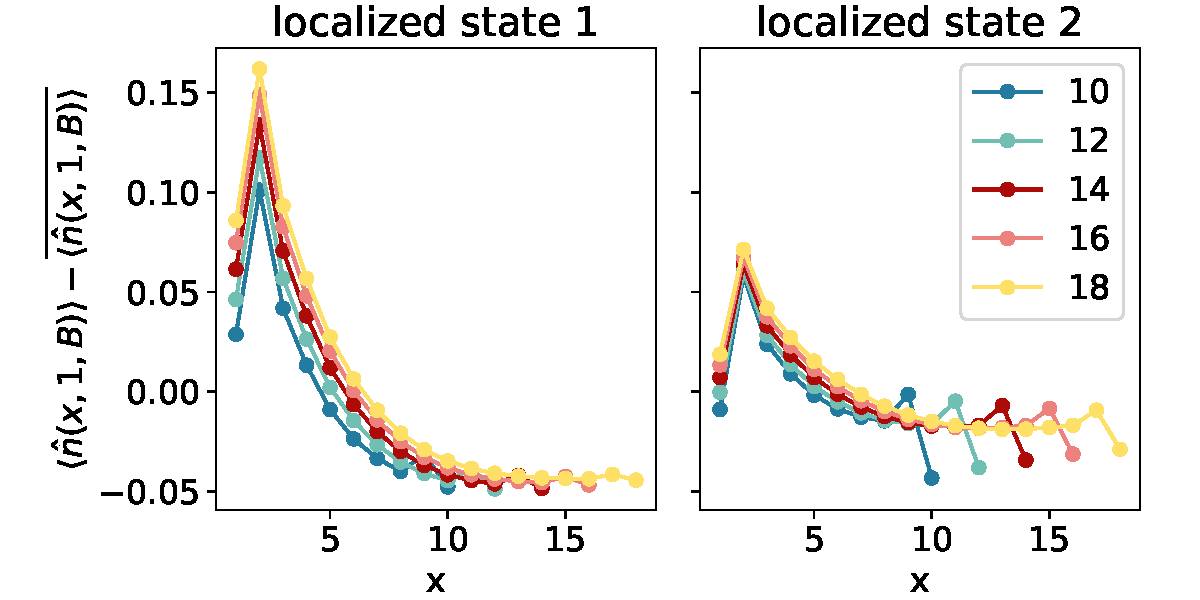
\includegraphics[width=1.\linewidth]{Picture/SI/SI_Comp2.pdf}
		\begin{overpic}[width=1.0\linewidth]{Picture/SI/SI_Comp2.pdf}
			\put(6,98){(a)}
			\put(54,98){(b)}
			% \put(7,54){(c)}
			\put(6,48){(c)}
			\put(54,48){(d)}
		\end{overpic}
		\caption{
		Average particle number $\langle \hat{n}(x, 1, B) \rangle $ and the deviations from the average $\langle \hat{n}(x, 1, B) \rangle - \overline{\langle \hat{n}(x, 1, B) \rangle}$ for the B sublattice at $y = 1$ boundary. 
		(a) The average particle number and the deviations from the average of the hybrid chiral skin correlated states (localized state 1). The $x$-axis is the location of the unit cell in the $x$ direction.
		(b) The average particle number and the deviations from the average of non-Hermitian many-body induced localized states (localized state 2).  The $x$-axis is the location of the unit cell in the $x$ direction.
		}
		\label{fig:15}
	\end{figure}
	The QWZ model is a topological insulator and exhibits edge states when the onsite energy $u$ lies within the range $-2 < u < 0$ and $0 < u < 2$. However, when the onsite energy is $u = -2.1$, the QWZ model is topologically trivial, and there are no edge states. 
	We apply gain to the boundary of a topologically trivial insulator and investigate whether multi-particle chiral skin modes and non-Hermitian many-body induced localized states can still arise.
	We study the hybrid chiral skin correlated states and non-Hermitian many-body induced localized states in larger system sizes. 
	We investigate the QWZ model with and without chiral skin modes, corresponding to onsite energies $u=-1.5$ and $u=-2.1$, respectively. The former is a topological insulator, while the latter is a trivial insulator. When inter-cell interactions $\hat{H}_{\text{inter}}$ are introduced, the model with chiral skin modes exhibits hybrid chiral skin correlated states, while the model without chiral skin modes exhibits non-Hermitian many-body induced localized states.
	We have shown that such localized states exist for system sizes up to $L_x = L_y = 9$ with the exact diagonalization method. To explore the localization in larger systems, we employ the Arnoldi method to compute the eigenstate with the largest imaginary eigenvalue. 
	We find that this eigenstate exhibits localization.
	The probability distribution of eigenstates and the average particle number of eigenstates for the hybrid chiral skin correlated states in larger systems are shown in Fig.\ref{fig:14} (a). 
	The probability distribution of eigenstates and the average particle number of eigenstates for non-Hermitian many-body induced localized states are shown in Fig.\ref{fig:14} (b). The results in Fig.~\ref{fig:14} show that these localized states still exist even in larger systems. Moreover, the hybrid chiral skin correlated states are more localized.


	We further investigate the behavior of hybrid chiral skin correlated states (labelled as localized state 1) and non-Hermitian many-body induced localized states (labelled as localized state 2) at different system sizes. Specifically, we study the average particle number $\langle \hat{n}(x, y, \alpha) \rangle$ and the deviation from average $\langle \hat{n}(x, y, \alpha) \rangle - \overline{\langle \hat{n}(x, y, \alpha) \rangle}$ along the $x$-direction for the $B$ sublattice at $y = 1$ boundary.
	As shown in Fig.~\ref{fig:15}, the peak amplitude of localized state 1 does not decrease as the system size increases, whereas the peak amplitude of localized state 2 decreases as the system size increases. This indicates that the behavior shown in Fig.\ref{fig:15} (a) is more localized than that in Fig.~\ref{fig:15} (b).
	Moreover, Fig.~\ref{fig:15} (c) and Fig.~\ref{fig:15} (d) reveal that the peak values of the deviation from average increases as system size increases for localized state 1, but remain nearly constant for localized state 2.
	hybrid chiral skin correlated states originate from many-body interactions that enhance the localization of topological corner states. 
	The energy splitting induced by many-body interactions further localizes these modes along both directions and confines them to the $B$ sublattice.
	In contrast, non-Hermitian many-body induced localized states arise from the combined effects of non-Hermiticity and many-body interactions. These states do not depend on the presence of localized topological corner states, called chiral skin modes, and therefore exhibit comparatively weaker localization.

	\subsubsection{The gain sites are not at the boundary}
	% \subsection{Robust to the location of dissipative sites}


	Chiral skin modes emerge when gain/loss unit cells are located at the boundaries of the lattice. 
	% These modes arise in topological insulators when edge states possess finite lifetimes.
	In contrast, when the gain is placed away from the lattice edges, chiral skin modes do not appear. In such cases, the introduction of many-body interactions does not lead to hybrid chiral skin correlated states, but instead gives rise to non-Hermitian many-body induced localized states. 
	Notably, the non-Hermitian many-body induced localized states exist even when gain is applied into the bulk of the system, and the eigenstates are not localized at the system's boundary.
	We consider a two-dimensional system of size $L_x = L_y = 9$, where gain is applied to the unit cells at $y = 3$. 
	The spectrum and eigenstates of the non-Hermitian Hamiltonians with or without $\hat{H}_{\text{inter}}$ many-body interactions are shown in Figs.~\ref{fig:10} (a) and (b), respectively. 
	The results in Fig.\ref{fig:10} indicate that no localized chiral skin modes emerge without interaction, since gain is not applied to the edge of the systems. 
	In the absence of many-body interaction, the eigenstate with the largest imaginary eigenvalue is a bulk state, as shown in Fig.~\ref{fig:10}(a3). However, when many-body interactions are present, the interaction-induced energy difference and non-Hermitian pumping give rise to non-Hermitian many-body induced localized states. In this case, the eigenstate localizes at the $B$ sublattice of the unit cells at $y = 3$.
	\begin{figure}[h]
		\centering
		\begin{overpic}[width=1.0\linewidth]{Picture/SI/SI_TwoExcitationSpectrum_NotEdge.pdf}
			\put(4,97){(a1)}
			\put(42,97){(b1)}
			% \put(7,54){(c)}
			\put(4,62){(a2)}
			\put(42,62){(b2)}
			\put(4,26){(a3)}
			\put(42,26){(b3)}
		\end{overpic}
		%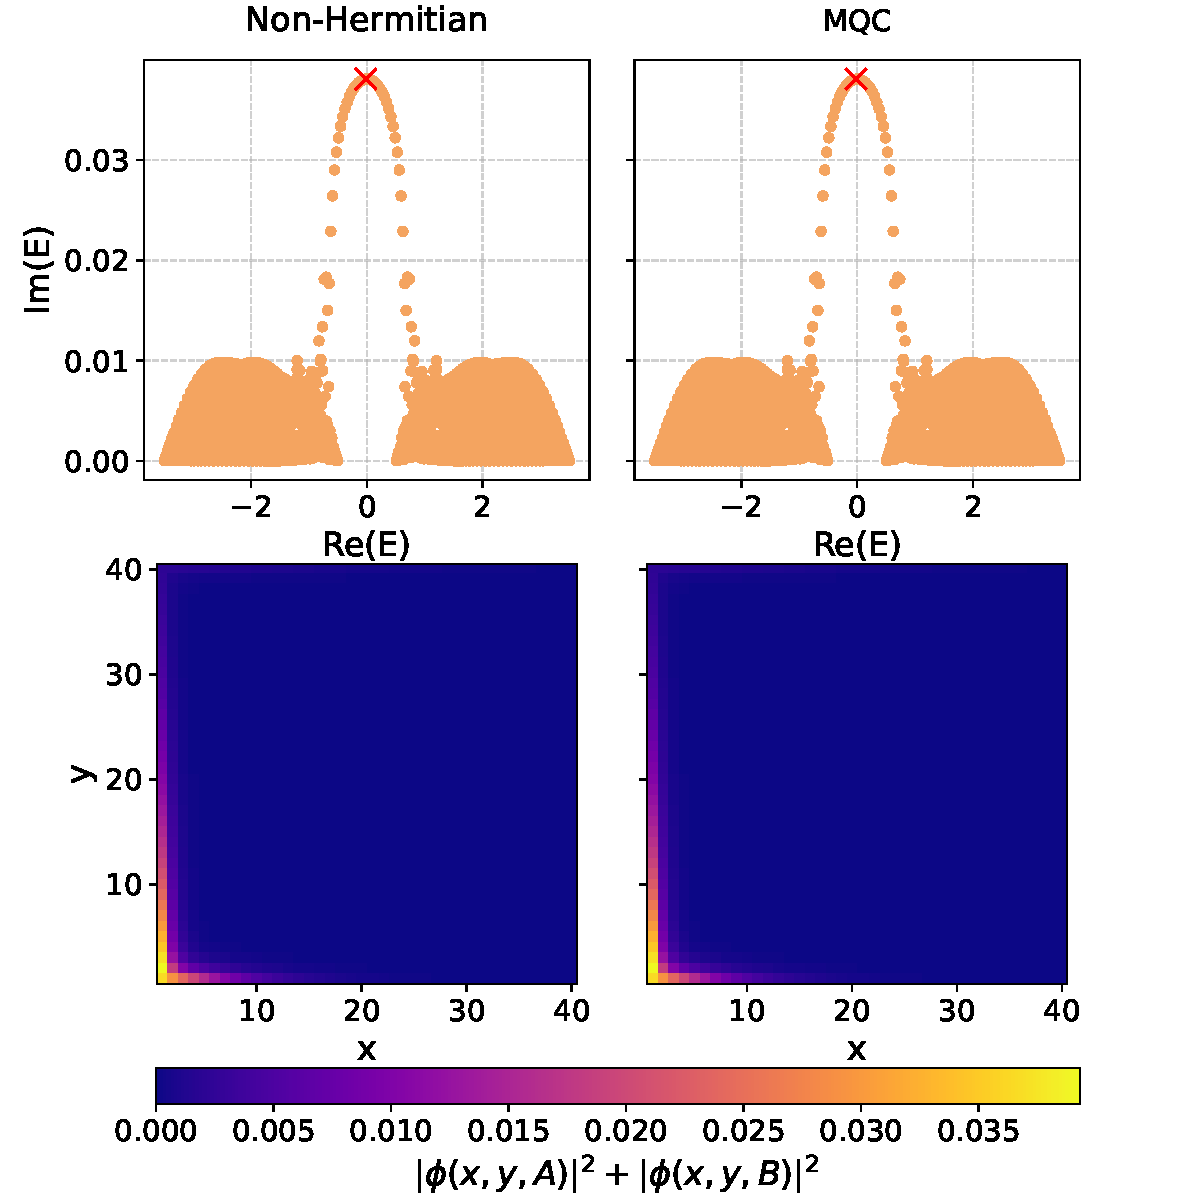
\includegraphics[width=1.\linewidth]{Picture/SingleExcitation_Comp.pdf}
		\caption{
		In the two-excitation subspace, the comparison of spectrum and eigenstates between non-Hermitan Hamiltonian with or without $\hat{H}_{\text{inter}}$ many-body interaction. The gain ($\gamma=0.2$) is applied to unit cells at $y=3$.
		(a1) The spectrum of a non-Hermitian Hamiltonian without interaction.
		(b1) The spectrum of a non-Hermitian Hamiltonian with interaction.
		(b2) The probability distribution of the eigenstates of a non-Hermitian Hamiltonian without interaction.
		(b2) The probability distribution of the eigenstates of a non-Hermitian Hamiltonian with interaction.
		(a3) The average particle number per lattice site for the eigenstate in (a2).
		(b3) The average particle number per lattice site for the eigenstate in (b2), which corresponds to non-Hermitian many-body interactions induced localized states.
		The system size is $L_x=L_y=9$, and the onsite potential is $u=-1.5$.
		}
		\label{fig:10}
	\end{figure} %label from y=1 and x=1?
    

	\subsection{The $\mathcal{P}_{x,y,\alpha}$ at different interaction strengths~\label{sec:AllP}}


	\begin{figure}[h]
		\centering
		\begin{overpic}[width=1.0\linewidth]{Picture/SI/SI_EvolveSpectrum2.pdf}
			\put(5,81){(a1)}
			\put(54,81){(a2)}
			\put(5,35){(a3)}
		\end{overpic}
		\caption{
		The spectrum and eigenstate in two-excitation subspace. The non-Hermitian gain ($\gamma=0.2$) is applied to unit cells at the $y=1$ boundary, and the many-body interaction is $\hat{H}_{\text{inter}}$. The system size for (a1-a3) is $L_x=L_y=7$. The onsite potential is $u=-1.5$.
		(a1) The spectrum of non-Hermitian many-body Hamiltonian.
		(a2) The probability distribution of the eigenstate of a non-Hermitian many-body Hamiltonian. 
		(a3) The average particle number per lattice site for the eigenstate.
		}
		\label{fig:17_2}
	\end{figure} %label from y=1 and x=1?

	The distinct spectral feature is also observable in digital quantum simulations. At this point, we choose the system size $L_x=L_y=7$, whose spectrum is similar to that in Fig.~\ref{fig:02} (a) ($L_x=L_y=9$). The spectrum and the eigenstate with the largest imaginary eigenvalue are shown in Fig.~\ref{fig:17_2}.
	%
	To study the hybrid chiral skin correlated states in different interaction strength $U_{\text{inter}}$, we introduce a measurable quantity which is compatible with the MQCs. % 我们定义了一种适合于量子电路监测的量度。
	In Fig.~\ref{fig:02_Supple}, we analyze the localization dynamics within the two-excitation subspace.
    We begin with the random excitation of two lattice sites to
	% by randomly exciting two lattice sites of the system to 
	study the time evolution of both the non-Hermitian Hamiltonian without and with the many-body interaction $\hat{H}_{\text{inter}}$. 
	% This evolution is implemented using the quantum circuit depicted in Fig.~\ref{fig:01}(a). 
	Subsequently, at time $t=60$, we measure the average particle number $\langle \psi_{t} \vert \hat{n}_{x,y,\alpha} \vert \psi_t \rangle$ of the final state $\psi_t$ at each lattice site ($\alpha=A,B$). We take the average over $N_{\text{samp}}=10^4$ experiments and statistically analyze the number of events where the expectation value $\langle \psi_{t} \vert \hat{n}_{x,y,\alpha} \vert \psi_t \rangle$ exceeds $1/(2L_x)$ at each lattice site
	\begin{equation}
		\mathcal{P}_{{x}, {y}, {\alpha}} = \sum^{N_{\text{samp}}} \mathbb{I}(\langle \psi_{t} \vert \hat{n}_{x,y,\alpha} \vert \psi_t \rangle > \frac{1}{2L_x}), \label{eq:NumbEvent}
	\end{equation}
	where $\mathbb{I}(X)$ is the indicator function, which is 1 (0) when $X$ is true (false).
	Our results demonstrate distinct localization behaviors under Hermitian and non-Hermitian many-body Hamiltonians. For the Hermitian case, when the system starts from an arbitrary localized two-excitation quantum state, the number of events $\mathcal{P}_{x,y,\alpha}$ at times $t=60$ exhibit a decreasing trend with increasing interaction strength $\vert U_{\text{inter}} \vert$. This suggests that stronger interactions drive the system toward delocalized states.
	In contrast, for the non-Hermitian case, the number of events $\mathcal{P}_{x,y,\alpha}$ at unit cell $(x,y)=(1,3)$ decreases with increasing interaction strength. the number of events at unit cells $(x,y)=(1,1),(1,2)$ first decreases and then increases (Fig.~\ref{fig:02_Supple}). 
	Therefore, the stronger many-body interaction can drive the system toward localized states in the presence of non-Hermiticity.
	This behavior is attributed to the presence of hybrid chiral skin correlated states, which ensure that regardless of the initial state, the system ultimately evolves into localized states and can be detected.
	When evolving from a random two-particle excited state, the system exhibits localization signals at the $B$ sites of the gain unit cells at time $t=60$.
	In about $88\%$ of the cases, the average particle number at one or more sites exceeds $1/(2L_x)$ (solid lines in Fig.~\ref{fig:02_Supple}).
	% A detailed analysis of $\mathcal{P}_{x,y,\alpha}$ for all lattice sites is provided in Appendix~\ref{sec:AllP}, which also supports the discussion here. 
	\begin{figure}[htbp]
		\begin{overpic}[width=0.95\linewidth]{picture2/Popu_Interaction.pdf}
		\end{overpic}
		\caption{The parameters $\mathcal{P}_{x,y,\alpha}$ at time $t=60$ for the non-Hermitian Hamiltonian with $\hat{H}_{\text{inter}}$ interaction under different interaction strengths. Gain is applied to $y=1$ boundary. The system size is $L_x=L_y=7$, and the onsite potential is $u=-1.5$. The number of randomly selected initial quantum states is $N_{\text{samp}}=10^4$.}
		\label{fig:02_Supple}
	\end{figure}



	We then investigate the behavior of $\mathcal{P}_{x,y,\alpha}$ for all lattice sites under different evolution times and interaction strengths $U_{\text{inter}}$. Specifically, we compute $\mathcal{P}_{x,y,\alpha}$ at times $t = 20$ and $t = 60$ under the dynamics governed by the Hamiltonians $\hat{H}_{\text{QWZ}} + \hat{H}_{\text{inter}}$ and $\hat{H}_{\text{QWZ}} + \hat{H}_{\text{inter}} + \hat{H}_{\text{im}}$ (Fig.~\ref{fig:appendixA_fig01}). 
	In the absence of non-Hermitian term, we observe that $\mathcal{P}_{x,y,\alpha}$ at all lattice sites consistently decreases as $\lvert U_{\text{inter}} \rvert$ increases, indicating that stronger interactions drive the system toward more delocalized quantum states. 
	In contrast, when non-Hermitian terms are present, a more intricate behavior emerges: while the parameter $\mathcal{P}_{x,y,\alpha}$ at $y\neq 1$ unit cells still decreases as interaction strength increases, 
	the parameter $\mathcal{P}_{x,y,\alpha}$ at $y=1$ unit cells first decreases then increases as interaction strength increases.
	This phenomenon arises from the emergence of hybrid chiral skin correlated states. The particles evolve to localized states regardless of the initial states. This localized states are then detected at site along $y=1$ boundary. The manifestation of this effect becomes more obvious at longer evolution times, and this effect has potential application in controlling exotic quantum states.
	%reflecting the system's approach toward a steady-state configuration.

	\begin{figure}[h]
		\centering
		%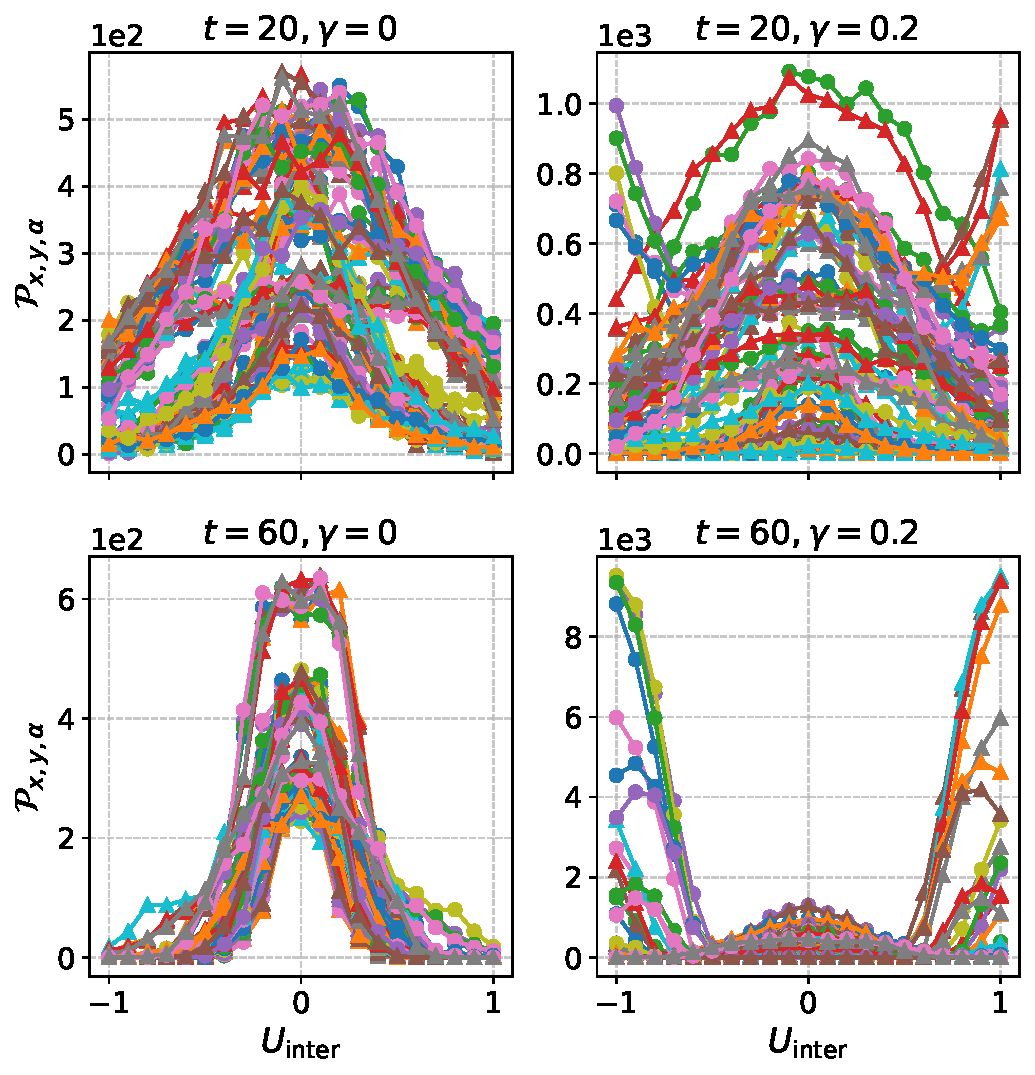
\includegraphics[width=1.\linewidth]{Picture/SI/SI_Popu_Interaction.pdf}
		\begin{overpic}[width=1.0\linewidth]{Picture/SI/SI_Popu_Interaction.pdf}
			\put(3,98){(a)}
			\put(50,98){(b)}
			\put(3,50){(c)}
			\put(50,50){(d)}
			% \put(49,54){(d)}
		\end{overpic}
		\caption{
		The parameters $\mathcal{P}_{x,y,\alpha}$ at times $t=20$ and $t=60$ under different interaction strengths $U_{\text{inter}}$. The initial quantum state is chosen as an arbitrary two-excitation state.
		(a) The results of many-body Hamiltonian without non-Hermitian gain at time $t=20$. 
		(b) The results of many-body Hamiltonian with non-Hermitian gain $\hat{H}_{\text{im}}$ ($\gamma=0.2$) at time $t=20$. 
		(c) The results of many-body Hamiltonian without non-Hermitian gain at time $t=60$. 
		(d) The results of many-body Hamiltonian with non-Hermitian gain $\hat{H}_{\text{im}}$ ($\gamma=0.2$) at time $t=60$. 
		Gain is applied to the $y = 1$ unit cell. The system size is $L_x=L_y=7$, and the onsite potential is $u=-1.5$. The number of randomly selected initial quantum states is $N_{\text{samp}}=10^4$.
		}
		\label{fig:appendixA_fig01}
	\end{figure}


	\subsection{The result with intra-cell many-body Hamiltonian~\label{sec:intra_cell_Hamiltonian}}
    
     \begin{figure}
    		\centering
    		\begin{overpic}[width=1.0\linewidth]{picture2/Pic_TwoExcitation_intra.pdf}
    			\put(6,88){(a)}
    			\put(54,88){(b)}
    			\put(6,44){(c)}
    			\put(54,44){(d)}
    		\end{overpic}
    		\caption{
    		The spectrum of the non-Hermitian Hamiltonian (a) without interaction and (b) with interaction $\hat{H}_{\text{intra}}$ in the two-excitation subspace. 
    			The eigenstate's average particle number $\langle \hat{n}(x,y,\alpha) \rangle$ of the eigenstate with the largest imaginary eigenvalue is shown in the inset. The non-Hermitian gain is applied to $y=1$ boundary. The energy of eigenstates is indicated by an orange cross in the spectrum. 
    			The two-particle correlation function $\langle \phi_i \vert \hat{n}^1 \hat{n}^2 \vert \phi_i \rangle$ between two particles of the eigenstate with the largest imaginary eigenvalue for non-Hermitian Hamiltonians (c) with or (d) without many-body interaction. In (b2), the positions where the two-particle correlation function exceeds 0.03 are marked with white circles.
    		  The system size is $L_x=L_y=9$ and the onsite potential is $u=-1.5$. The non-Hermitian gain is applied to $y=1$ boundary. 
    		}
    		\label{fig:02a_intra}
    	\end{figure}
        
    We also consider the intra-cell many-body interaction
    \begin{equation}
        \hat{H}_{\text{intra}} = \sum_{{x}=1}^{L_{x}-1} \sum_{{y}=1}^{L_{y}}  U_{\text{intra}} \hat{n}_{{x}, {y}, A} \hat{n}_{{x}, {y}, B}, \label{eq:intra_cellHamil}
    \end{equation}
    where $\hat{n}_{{x},{y},\alpha}=\hat{c}_{x,y,\alpha}^{\dagger}\hat{c}_{x,y,\alpha}$ denotes the number operator at $\alpha$ sublattice of the unit cell with position (${x},{y}$).
    In the two-excitation subspace, the spectrum and average particle number at each lattice site of the gain non-Hermitian Hamiltonians 
	%both in the absence and presence of inter-cell interaction $\hat{H}_{\text{inter}}$ 
	are shown in Fig.~\ref{fig:02a_intra}. Figs.~\ref{fig:02a_intra} (a-b) show the energy spectrum for the non-Hermitian Hamiltonian without and with the intra-cell many-body Hamiltonian (Eq.~\ref{eq:intra_cellHamil}). 
    The inset of the Figs.~\ref{fig:02a_intra} (a) and (b) show the average particle number at each lattice site for the eigenstate $\langle \hat{n}(x,y,\alpha) \rangle$.

   Under the intra-cell interaction Hamiltonian $\hat{H}_{\text{intra}}$ ($U_{\text{intra}}=1.0$), the spectrum of the Hamiltonian in the two-excitation subspace shows that although the symmetry of the spectrum with respect to $\mathrm{Re}(E)=0$ is broken, the eigenstate with the largest imaginary eigenvalue retains a chiral skin mode. 
	The difference exists solely in the particle number occupation at each lattice site. In contrast, when many-body interaction $\hat{H}_{\text{inter}}$ is introduced, the many-body interaction $\hat{H}_{\text{inter}}$($U_{\text{inter}}=1.0$) alters eigenvalue distribution and eigenstate localization pattern. Moreover,
    the correlation patterns (Figs.~\ref{fig:02a_intra} (c) and (d)) remain qualitatively similar between the non-interacting case and the intra-cell interaction case, and it is different from the strong spatial correlation patterns for the inter-cell interaction case. 

	\subsection{The hybrid chiral skin correlated states exist in a dissipative Hamiltonian.~\label{sec:appendicD_loss}}
	\begin{figure}[h]
		\centering
		\begin{overpic}[width=1.0\linewidth]{Picture/SI/SI_TwoExcitationSpectrum_loss.pdf}
			\put(4,97){(a1)}
			\put(44,97){(b1)}
			% \put(7,54){(c)}
			\put(4,62){(a2)}
			\put(44,62){(b2)}
			\put(4,26){(a3)}
			\put(44,26){(b3)}
		\end{overpic}
		%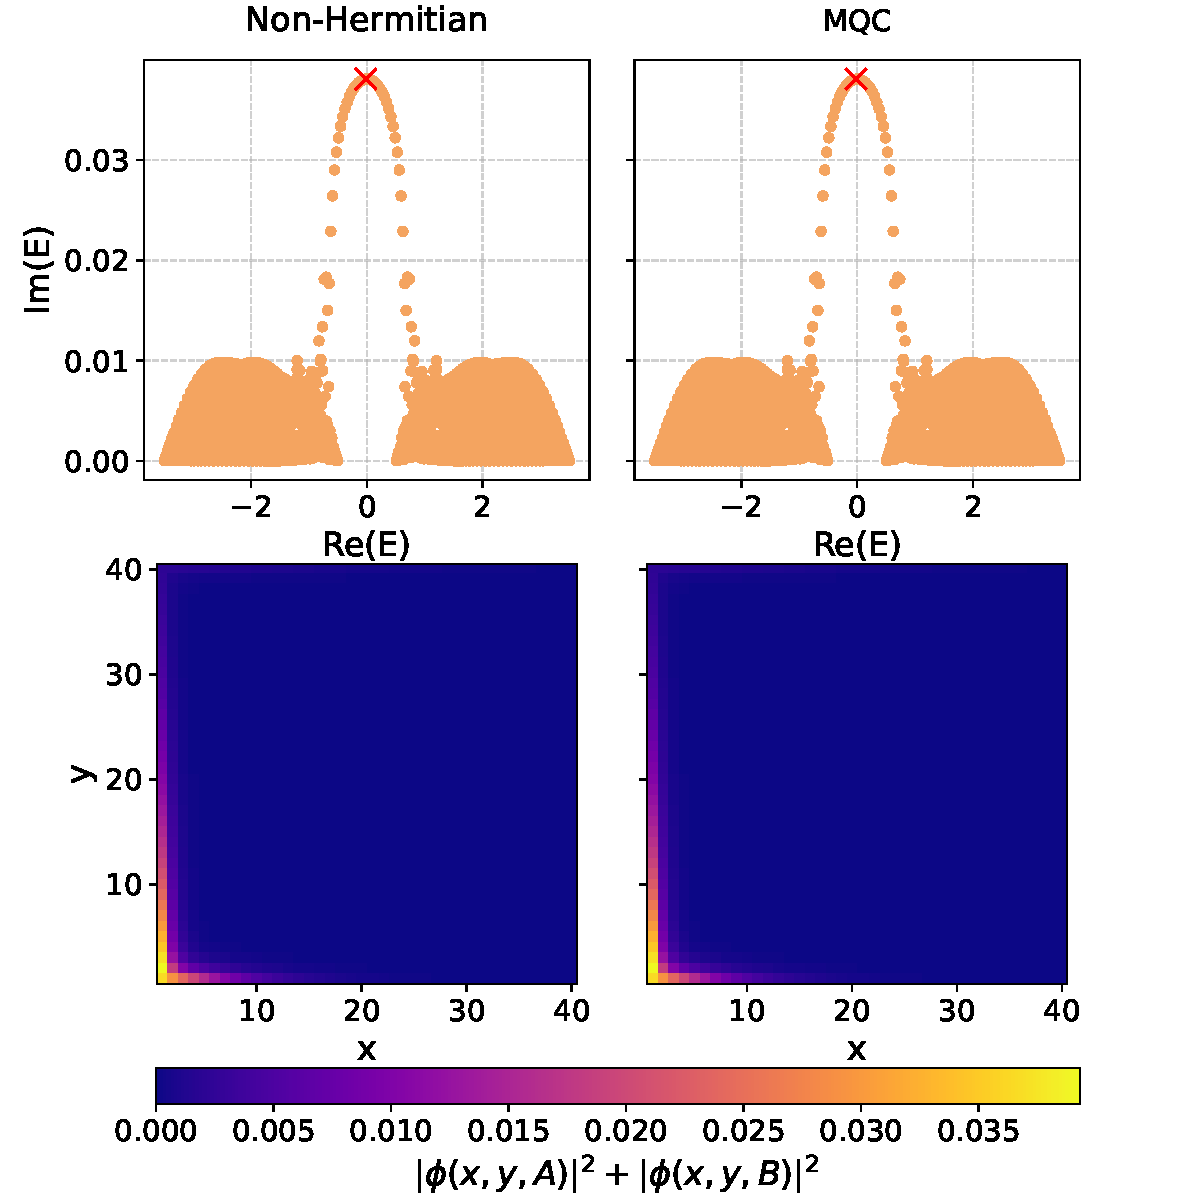
\includegraphics[width=1.\linewidth]{Picture/SingleExcitation_Comp.pdf}
		\caption{
		In the two-excitation subspace, the comparison of spectrum and eigenstates between non-Hermitan Hamiltonian with or without $\hat{H}_{\text{inter}}$ many-body interaction. The non-Hermitian dissipation ($\gamma=-0.2$) is applied to unit cells at the $y=1$ boundary.
		(a1) The spectrum of a non-Hermitian Hamiltonian without interaction.
		(b1) The spectrum of a non-Hermitian Hamiltonian with interaction.
		(a2) The probability distribution of the eigenstates of a non-Hermitian Hamiltonian without interaction.
		(b2) The probability distribution of the eigenstates of a non-Hermitian Hamiltonian with interaction.
		(a3) The average particle number per lattice site for the eigenstate in (a2).
		(b3) The average particle number per lattice site for the eigenstate in (b2), which corresponds to the hybrid chiral skin correlated states in dissipative systems.
		The system size is $L_x=L_y=9$, and the onsite potential is $u=-1.5$.
		}
		\label{fig:13}
	\end{figure} %label from y=1 and x=1?
	
	To gain deeper insight into the physical mechanism of the hybrid chiral skin correlated states, we have primarily focused on systems with gain in the preceding analysis.  
	Note that the hybrid chiral skin correlated states exist even when only dissipative terms are present.
	According to the mechanism described above, the dissipative term pumps particles out of the subspace $\mathscr{H}_{\text{gain}}$ during time evolution.
	%the time evolution of dissipative term can be interpreted as pumping particles out of subspace $\mathscr{H}_{\text{gain}}$. 
	This process seems to indicate that dissipation does not induce localization, because particles are pumped out from subspace $\mathscr{H}_{\text{gain}}$ and do not accumulate in this subspace.

	The time evolution of the  non-Hermitian Hamiltonian drives the system toward the eigenstate with the largest imaginary eigenvalue, which is the delocalized state.
	We consider the time-reversed evolution operator $e^{\mathrm{i}(\hat{H} + \hat{H}_{\text{im}})t}$. The time-reversed evolution of the non-Hermitian term pumps particles into the subspace $\mathscr{H}_{\text{gain}}$. After evolving under the reversed dynamics for a sufficiently long time, the quantum state evolves to a localized state.
	Figs.~\ref{fig:13} (a1) and (b1) show the spectrum for a dissipative non-Hermitian Hamiltonian with or without many-body interaction. 
	In Fig.~\ref{fig:13} (a2) and (b2), the probability distributions of the eigenstate with the smallest imaginary eigenvalue (orange cross in Figs.~\ref{fig:13} (a1) and (b1)) is shown.
	Figs.~\ref{fig:13} (a3) and (b3) show the average particle number at each lattice site for the eigenstate. 
	The results show that the eigenstate with the smallest imaginary eigenvalue is localized, and this eigenstate is the steady state of long time-reversed evolution. 

	Moreover, gain non-Hermitian Hamiltonians and loss non-Hermitian Hamiltonians can be transformed to each other under a combination of reflection $\mathcal{M}_x$ and complex conjugate transformation $\mathcal{K}$.
	This symmetry reveals the mapping between Fig.\ref{fig:02} (c) and Fig.\ref{fig:13}. Specifically, the state localized at the left bottom corner in Fig.\ref{fig:02} (c), while the state localized at the left top corner in Fig.\ref{fig:13} (a3) and (b3).
	%, illustrating the spatial inversion under $\mathcal{M}_x$.
	Finally, note that both time evolution and time-reversed evolution of non-Hermitian Hamiltonians can, in principle, be implemented in MQCs with quantum gates. To simulate the evolution of a non-Hermitian Hamiltonian with loss (gain), we can initialize the ancillary qubit to state $\ket{0}$ ($\ket{1}$), and then postselect the quantum trajectories with measurement outcomes $\ket{0}$ ($\ket{1}$). This approach enables experimental realization and detection of hybrid chiral skin correlated states of dissipative systems in the MQCs.


	\subsection{The construction of non-Hermitian many-body Hamiltonians based on MQCs~\label{sec:scheme_method}}

	We propose a general scheme to realize the evolution of gain/loss non-Hermitian Hamiltonian in the MQCs.
	The general form of such Hamiltonians contains both Hermitian and non-Hermitian components:
	\begin{equation}
		\hat{H} = \hat{H}_0 +\hat{H}_{\text{im}}. \label{eq:non-hermitian}
	\end{equation}
	The non-Hermitian part $\hat{H}_{\text{im}}$ is the sum of gain/loss energy on each site, which holds imaginary onsite energy, such as $\hat{H}_{\text{im}} = \sum_{i\in \text{dissi}} \mathrm{i}\tilde{\gamma} \hat{c}_i^{\dagger} \hat{c}_i$ for gain/loss energy. 
	% 上面这段描述多余吗？
	After Jordan-Wigner transformation, the Hamiltonian of fermion system can be implemented through the MQCs, where each lattice site is encoded in a qubit. 
	%The details of Jordan-Wigner transformation can be found in Methods.  
	Throughout this work, the qubit state $\ket{0}$ ($\ket{1}$) indicates the absence (presence) of a fermion at the lattice site.


	The digital quantum computer can be used to simulate the fermionic system. 
	A negative sign will appear when exchanging the fermion at different sites, but qubits do not have this property. 
	% 为了满足费米子算符的对易关系，我们引入一个链算符
	To preserve the fermionic commutation relations, we introduce a string operator defined as
	\begin{equation}
		P_i = \otimes_{j=1}^i\hat{\sigma}^z_j.
	\end{equation}
	%基于该链算符，采用上升算符$\sigma^+=(\sigma^x+\mathrm{i}\sigma^y)/2$和下降算符$\sigma^-=(\sigma^x-\mathrm{i}\sigma^y)/2$表示费米子产生湮灭算符为：
	Using this string operator $P_i$, the fermionic creation and annihilation operators can be expressed in terms of the raising operator $\hat{\sigma}^+=(\hat{\sigma}^x+\mathrm{i}\hat{\sigma}^y)/2$ and the lowering operator $\hat{\sigma}^-=(\hat{\sigma}^x-\mathrm{i}\hat{\sigma}^y)/2$ as follows:
	\begin{equation}
		\begin{split}
			\hat{c}_i = P_i \otimes \hat{\sigma}^{-}\otimes (\otimes_{j=i+1}\hat{\sigma}^0_j)\\
			\hat{c}_i^{\dagger} = P_i \otimes \hat{\sigma}^{+}\otimes (\otimes_{j=i+1}\hat{\sigma}^0_j),
		\end{split}
	\end{equation}
	where $\hat{\sigma}^{x,y,z}$ represent the Pauli matrices and $\hat{\sigma}^0$ represents $2\times 2$ identity matrix. 
	% This transformation is called Jordan-Wigner transformation. 
	
	In general, the underlying interesting phenomena are uncovered through the evolution dynamics in the MQCs. The evolution of non-Hermitian Hamiltonian $U(t) = e^{-\mathrm{i}(\hat{H}_0 + \hat{H}_{\text{im}})t}$ is realized by alternately implementing $\mathrm{d} t$ time evolution of the Hermitian part $U_0(\mathrm{d}t)=e^{-\mathrm{i}\hat{H}_0 t}$ and $\mathrm{d} t$ time evolution of non-Hermitian part. 
	% The effect of $U_0(\mathrm{d}t)$ on the input qubit is shown in the middle of Fig.~\ref{fig:01}(a).
	The evolution of the Hermitian part $\hat{H}_0$ is decomposed via Trotter expansion, and each of them is a multi-qubit gate. 
	% The evolution of the Hermitian part can be realized through quantum gates. 
	% The evolution can be expanded through Trotter expansion, and the evolution of each hopping term including many-body interaction is a multi-qubit quantum gate. 
	The time evolution of the non-Hermitian part $\hat{H}_{\text{im}}$ is implemented through generalized measurements $M_i$.
	%, as shown in Sec.\ref{sec:method}. 
	Here, the generalized measurements are defined as a set of Kraus operators $\{M_{i,\beta},\beta=0,\pm \}$, which are a completely positive trace-preserving map. Without any postselection, the map is defined as
	$\varepsilon(\rho) = \sum_{\beta} M_{i, \beta} \rho M_{i, \beta}^{\dagger}$, and $\rho$ is the density matrix of the fermionic system.
	The generalized measurements on the ith site are defined as
	\begin{align}
		&M_{i,\pm} = \sqrt{\frac{1}{2+(e^{\gamma \mathrm{d} t} - e^{-\gamma \mathrm{d} t})^2}} (1 + (e^{\pm \gamma \mathrm{d} t}-1) \hat{c}_i^{\dagger} \hat{c}_i),\\
		&M_{i,0} = \sqrt{\frac{(e^{\gamma \mathrm{d} t} - e^{-\gamma \mathrm{d} t})^2}{2+(e^{\gamma \mathrm{d} t} - e^{-\gamma \mathrm{d} t})^2}} c_i^{\dagger},
	\end{align}
	which satisfy the trace-preserving condition $\sum_{\beta} M_{i,\beta}^{\dagger} M_{i,\beta}=\mathrm{I}$. 
	Note that the measurement interval $\mathrm{d}t$ is a parameter in the generalized measurements. 
	Although not all operations can be implemented, the measurements above can be realized through projection measurements in an enlarged Hilbert space, as guaranteed by Naimark's theorem~\cite{coecke2008povms,nielsen2001quantum}. As a result, our scheme can be implemented with current experimental techniques through the introduction of auxiliary qubits.
	The dissipative non-Hermitian Hamiltonian with onsite loss $-\mathrm{i}\gamma$ can be realized through postselecting $M_{i,-}$, while the non-Hermitian Hamiltonian with onsite gain $\mathrm{i}\gamma$ can be realized through postselecting $M_{i,+}$. 
	% under what condition, it is a projective measurement!(no) Explain our measurement. 
	
	Our measurement scheme postselects the outcome of $M_{i,-}$ for dissipative non-Hermitian, which maps the state $\vert \psi \rangle$ to $M_{i,-} \vert \psi \rangle/\Vert M_{i,-} \vert \psi \rangle \Vert$ with a probability of $\Vert M_{i,-} \vert \psi \rangle \Vert^2$. 
	%If the Hermitian part $\hat{H}_0$ and the non-Hermitian part $\hat{H}_{\text{im}}$ are not commutative, 
	The parameter of measurements should satisfy $\gamma \mathrm{d} t \ll 1$.
	The realization of generalized measurements $\{M_{i,\beta}, \beta=\pm,0\}$ is difficult. However, measurements $M_{i,+}$ and measurements $M_{i,-}$ can be realized though one ancillary qubit. We first apply a two-qubit unitary gate to the qubit and the ancillary qubit, which is
	\begin{equation}
		U_{\text{M}} = \begin{pmatrix}
		  1 & 0 & 0 & 0\\
		  0 & e^{-\gamma \dif t} & \sqrt{1-e^{-2 \gamma \dif t}} & 0\\
		  0 & -\sqrt{1-e^{-2 \gamma \dif t}} & e^{-\gamma \dif t} & 0\\
		  0 & 0 & 0 & 1
		\end{pmatrix}.
	\end{equation}
	If the ancillary qubit is prepared on state $\ket{0}$($\ket{1}$), the measurement $M_{i,-}$($M_{i,+}$) can be realized when the measurement on the ancillary qubit gives $\ket{0}$ ($\ket{1}$) results. 

	To implement the measurements $M_{i,-}$, we initialize the ancillary qubit in the state $\ket{0}$. For an initial state $\alpha \ket{0} + \beta \ket{1}$, the joint state after applying the unitary operation $U_M$ become
	% The state after applying $U_M$ is 
	%Suppose the initial state $\alpha \ket{0} + \beta \ket{1}$, after applying the $U_M$, we get
	\begin{equation}
		(\alpha \ket{0} + \beta e^{-\gamma \mathrm{d}t} \ket{1}) \otimes \ket{0} - \beta \sqrt{1-e^{-2\gamma\mathrm{d}t}} \ket{0} \ket{1}.
	\end{equation}
	Subsequent projection of the ancillary qubit onto $\ket{0}$ yields the unnormalized system state $\alpha \ket{0} + \beta e^{-\gamma \mathrm{d}t} \ket{1}$. 
	Conversely, for the implementation of $M_{i,+}$, the ancilla is initialized to $\ket{1}$. The joint state after applying $U_M$ is
	\begin{equation}
		(\alpha e^{-\gamma \mathrm{d}t} \ket{0} + \beta  \ket{1}) \otimes \ket{1} + \alpha \sqrt{1-e^{-2\gamma\mathrm{d}t}} \ket{1} \ket{0}.
	\end{equation}
	Projective measurement of the ancilla in $\ket{1}$ then collapses the system to $\alpha e^{-\gamma \mathrm{d}t} \ket{0} + \beta  \ket{1}$.
	%After projecting the ancillary qubit to state $\ket{1}$, we get state $\alpha e^{-\gamma \mathrm{d}t} \ket{0} + \beta  \ket{1}$.
	Through the two-qubit gates and the $\hat{\sigma}_z$ measurements on the ancillary qubit, we can realize the time evolution of non-Hermitian Hamiltonian $e^{-\mathrm{i} (\pm \mathrm{i} \hat{c}_i^{\dagger}\hat{c}_i) \mathrm{d}t}$.

	Based on the realization of $\hat{H}_0$ and $\hat{H}_{\text{im}}$ in the MQCs individually, the whole evolution process is to first perform the unitary evolution of $\hat{H}_0$ on all sites and then the generalized measurements on all dissipative sites. It is described as $E=(\prod_{i\in \text{dissi}} M_{i,-}) U_{0}(\mathrm{d} t),U_{0}(\mathrm{d}t)=e^{-\mathrm{i}\hat{H}_0 \mathrm{d}t}$.
	Instead of performing all measurements on gain/loss sites, our scheme performs the measurement on each gain/loss site with a classical probability $p\in(0,1]$. 
	Without loss of generality, we set the measurement probability to $p=1$. 
	%, see Fig.~\ref{fig:monitoredquantumcircuit}(a). 
	Then we obtain a probabilistic quantum circuit operator, and the process of performing it on an initial state $\vert \psi \rangle$ is described by
	\begin{equation}
		\frac{E(p,r) \vert \psi \rangle}{\Vert E(p,r) \vert \psi \rangle \Vert} = \frac{(\prod_j M_{j,-}^{r_j}) \cdot U_0(\mathrm{d}t)}{\Vert (\prod_j M_{j,-}^{r_j}) \cdot U_0(\mathrm{d}t) \vert \psi \rangle \Vert} \vert \psi \rangle,
	\end{equation}
	where $U_0(\mathrm{d} t) = e^{-\mathrm{i}\hat{H}_0 \mathrm{d} t}$ and $r_j$ = 0 or 1 with a probability of $1-p$ and $p$, respectively. So $N$-layer MQC with a probability of $p$ is defined as
	\begin{equation}
		E_N(p,\{r\}) = E(p, r_N) \circ E(p, r_{N-1}) \circ \cdots \circ E(p, r_1).
	\end{equation}
	The effective Hamiltonian $\hat{H}_{\text{eff}}^{(N)}$ of \textit{N}-layer quantum circuit~\cite{fleckenstein2022non} is 
	\begin{equation}
		\hat{H}^{(N)}_{\text{eff}} = \hat{H}_0 + \sum_{i\in \text{dissi} } (-\mathrm{i} p\gamma \hat{c}_i^{\dagger} \hat{c}_i) + \mathcal{O}(\nu\mathrm{d} t) + \mathcal{O}(1/\sqrt{N}).\label{eq:H_scheme1}
	\end{equation}
	% The connection between the effective Hamiltonian $\hat{H}_{\text{eff}}^{(N)}$ and its non-Hermitian counterpart is derived in Methods~\ref{sec:method}.

	After evolving the circuits for a sufficiently long time, the topological properties, including edge states and corner states~\cite{zou2021observation,shen2025observation}, can be probed. These features are revealed by measuring the average number operator at the end of the circuit, which corresponds to local $\hat{\sigma}_z$ measurements. 
	% The details have been shown in the right part of Fig.~\ref{fig:01} (a).


	The paradigmatic Hamiltonians with many-body interactions are
	\begin{widetext}
		\begin{align}
			\hat{H}_{\text{inter}} = &\sum_{{x}=1}^{L_{x}-1} \sum_{{y}=1}^{L_{y}}  U_{\text{inter}} \left(\hat{n}_{{x}, {y}, A}+\hat{n}_{{x}, {y}, B}\right) \left(\hat{n}_{{x}+1, {y}, A}+\hat{n}_{{x}+1, {y}, B}\right)\notag\\
			& + 
			\sum_{{x}=1}^{L_{x}} \sum_{{y}=1}^{L_{y}-1}  U_{\text{inter}} \left(\hat{n}_{{x}, {y}, A}+\hat{n}_{{x}, m_y, B}\right) \left(\hat{n}_{{x}, {y}+1, A}+\hat{n}_{{x}, {y}+1, B}\right),\\
			% \hat{H}_{\text{intra}} =& \sum_{{x}=1}^{L_{x}-1} \sum_{{y}=1}^{L_{y}}  U_{\text{intra}} \hat{n}_{{x}, {y}, A} \hat{n}_{{x}, {y}, B},
		\end{align}
	\end{widetext}
	where $\hat{n}_{{x},{y},\alpha}=\hat{c}_{x,y,\alpha}^{\dagger}\hat{c}_{x,y,\alpha}$ denotes the number operator at $\alpha$ sublattice of the unit cell with position (${x},{y}$).
	The many-body interaction $\hat{H}_{\text{inter}}$ can be effeciently implemented in MQCs. Each interaction term after Jordan-Wigner transformations can be realized below.

	To implement the time evolution of the Hermitian Hamiltonian $\hat{H}_{\text{QWZ}}$ and $\hat{H}_{\text{inter}}$ with elementary quantum gates, we employ Trotter decomposition for the Hamiltonian. For instance, the time evolution of the hopping term $e^{-\mathrm{i}  (\hat{c}_{1,2,A}^{\dagger} \hat{c}_{1,1,A} +h.c.)\mathrm{d} t/2}$ can be expressed, after the Jordan-Wigner transformation, as $e^{-\mathrm{i} (\hat{\sigma}_{1,2,A} \hat{\sigma}^z_{1,1,B}\hat{\sigma}_{1,1,A}^{-} +h.c.)\mathrm{d} t /2}$, which corresponds to a three-qubit quantum gate.
	The time evolution of interaction term $ U_{\text{inter}} \hat{n}_{1, 1, A} \hat{n}_{2,1,A}$ after Jordan-Wigner transformation is $U_{\text{inter}} (\hat{\sigma}^z_{1,1,A}+1)(\hat{\sigma}^z_{2,1,A}+1)/4$. The evolution of this interaction term can be realized through two-qubit gates 
	\begin{equation}
		e^{-\mathrm{i} U_{\text{inter}} (\hat{\sigma}^z_{1,1,A}+1) (\hat{\sigma}^z_{2,1,A}+1) \mathrm{d}t/4 }. \notag
	\end{equation}
	% \subsection{single-excitation subspace}

        \begin{figure*}[htbp]
		\hfill
		\begin{minipage}[b]{1.\textwidth}
			% 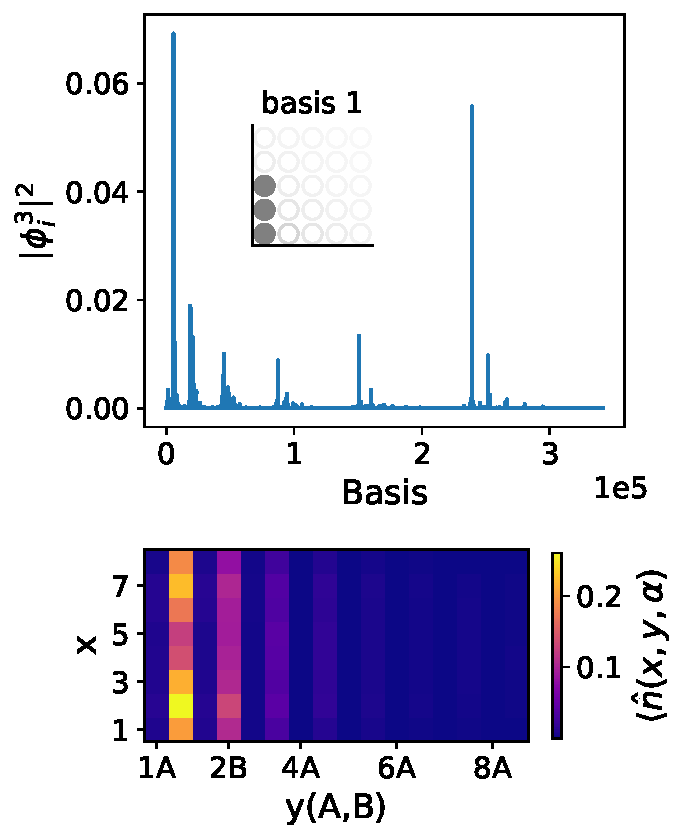
\includegraphics[width=1.\linewidth]{Picture/SI/SI_ThreeExcitationSize8.pdf}
			\begin{overpic}[width=0.345\linewidth]{Picture/SI/SI_ThreeExcitationSize8.pdf}
				% \put(-165,102){(a1)}
				% \put(-165,52){(b1)}
			\end{overpic}
			% \caption{图片4说明}
			% \label{fig:img4}
			\begin{overpic}[width=0.635\linewidth]{Picture/3D_Mechanism_inter.pdf}
				\put(-45,67){(a)}
				\put(1,67){(b)}
				% \put(3,52){(b)}
			\end{overpic}
		\end{minipage}
		\caption{
		(a) The probability distribution and average particle number of the eigenstate with the largest imaginary eigenvalue atsystem size $L_x=L_y=8$. This state corresponds to the hybrid chiral skin correlated states in the three-excitation subspace.
		(b) The spectrum and eigenstate's average particle number $\langle \hat{n}(x,y,\alpha) \rangle$ of non-Hermitian Hamiltonian without many-body interaction in the three-excitation subspace. 
		The complex energy of the eigenstate is marked by an orange cross in the spectrum. 
		(c) The three-particle correlation function $\langle \phi_i \vert \hat{n}^1_{x,y,\alpha} \hat{n}^2_{x,y,\alpha} \hat{n}^3_{x,y,\alpha} \vert \phi_i \rangle$ bwteen three particles of the eigenstate with the largest imaginary eigenvalue of non-Hermitian Hamiltonians with interaction $\hat{H}_{\text{inter}}$. The system size is $L_x=L_y=5$ and the onsite potential is $u=-1.5$. The non-Hermitian gain is applied to $y=1$ boundary.
		}
		\label{fig:03}
	\end{figure*}
    
	In this way, the Hermitian part of the system is composed of $\hat{H}_0=\hat{H}_{\text{QWZ}}+\hat{H}_{\text{inter}}$. The non-Hermitian term $\hat{H}_{\text{im}}$ is depicted below Eq.~\eqref{eq:non-hermitian}. The former discussions have stated that the non-Hermitian QWZ model can give the chiral skin modes, which are beyond the conventional skin modes in the one-dimensional lattice~\cite{nakamura2023universal, ma2024non,schindler2023hermitian}. Such phenomena can be observed easily on the classical platforms. However, when the many-body interactions are contained, the classical platforms are not able to handle them due to a lack of enough Hilbert space. The MQC provides an ideal platform to explore the effect of the many-body interactions in a convenient way.


	\subsection{The mechanism in the three-excitation subspace~\label{sec:three_excitation}}

	\begin{figure*}
		% 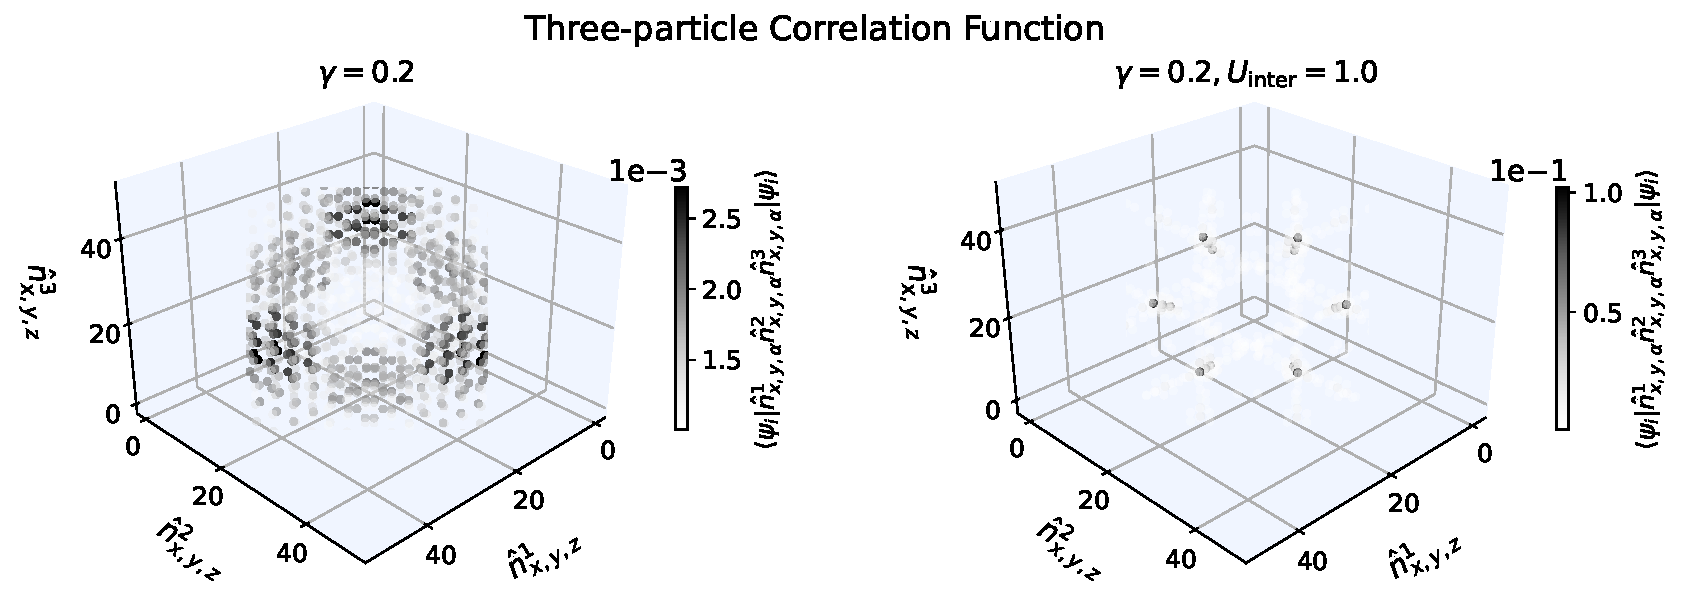
\includegraphics[width=0.98\linewidth]{Picture/CorrelationMap_3P.pdf}
		\begin{minipage}[b]{1.\textwidth}
			% 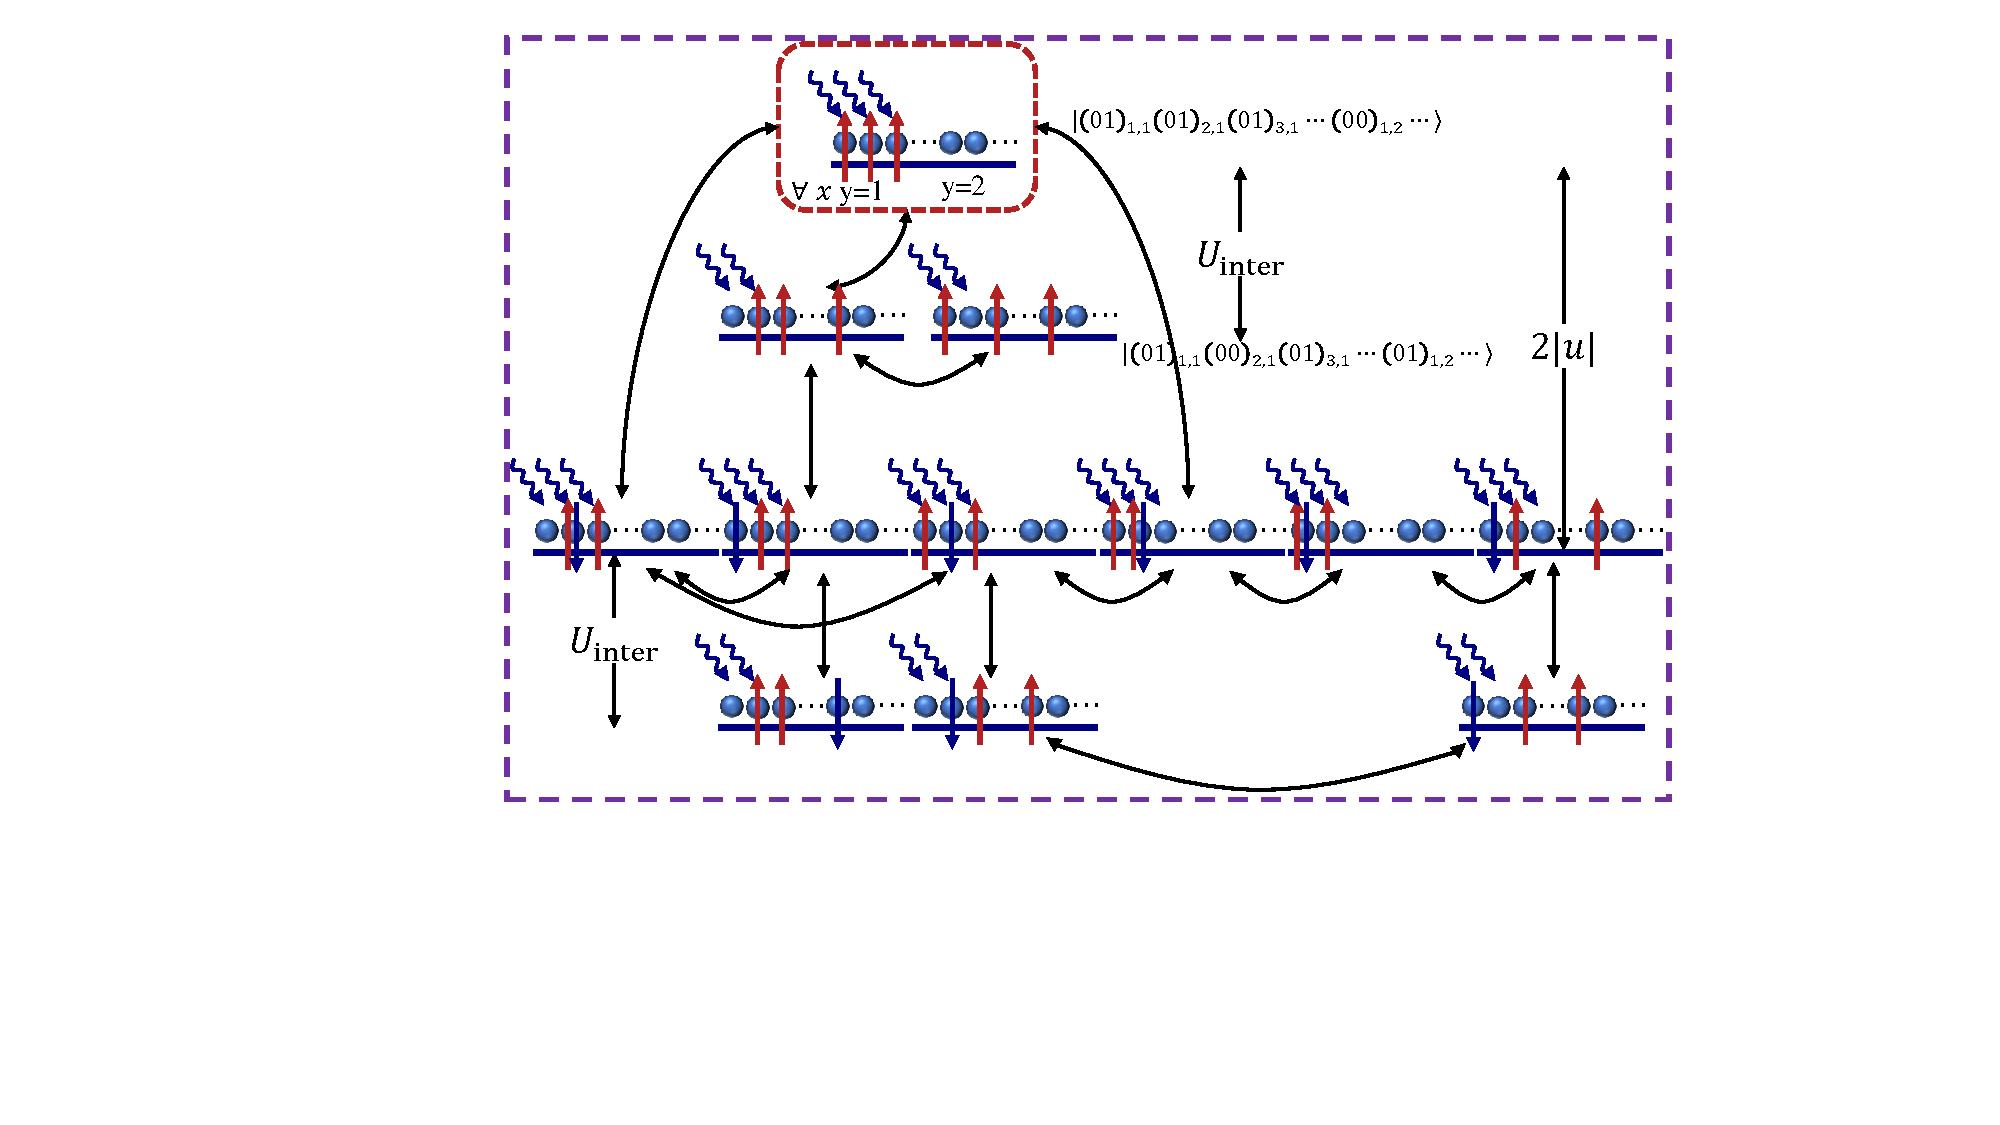
\includegraphics[width=\textwidth]{Picture/3D_Mechanism_inter.pdf}
			% 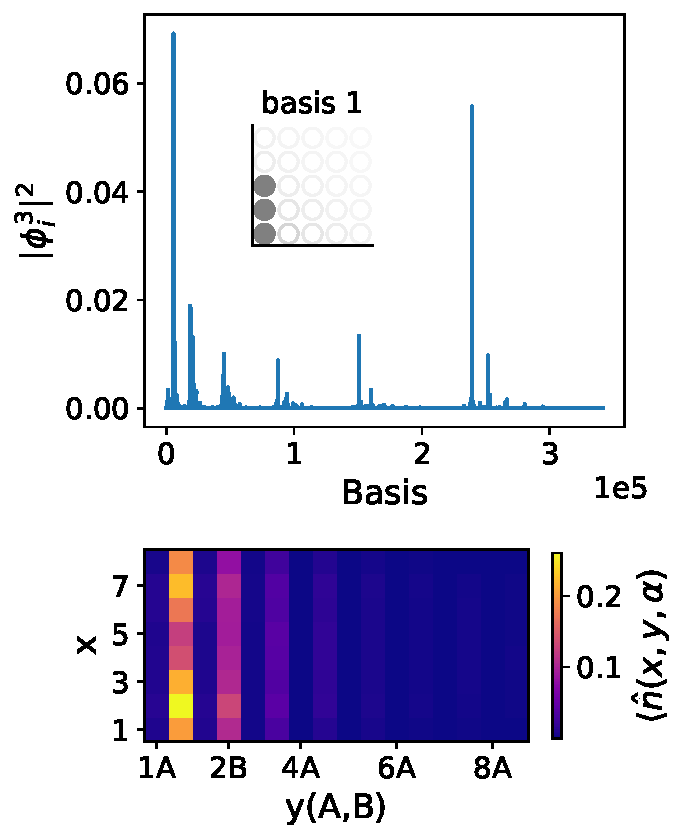
\includegraphics[width=0.29\linewidth]{Picture/SI/SI_ThreeExcitationSize8.pdf}
			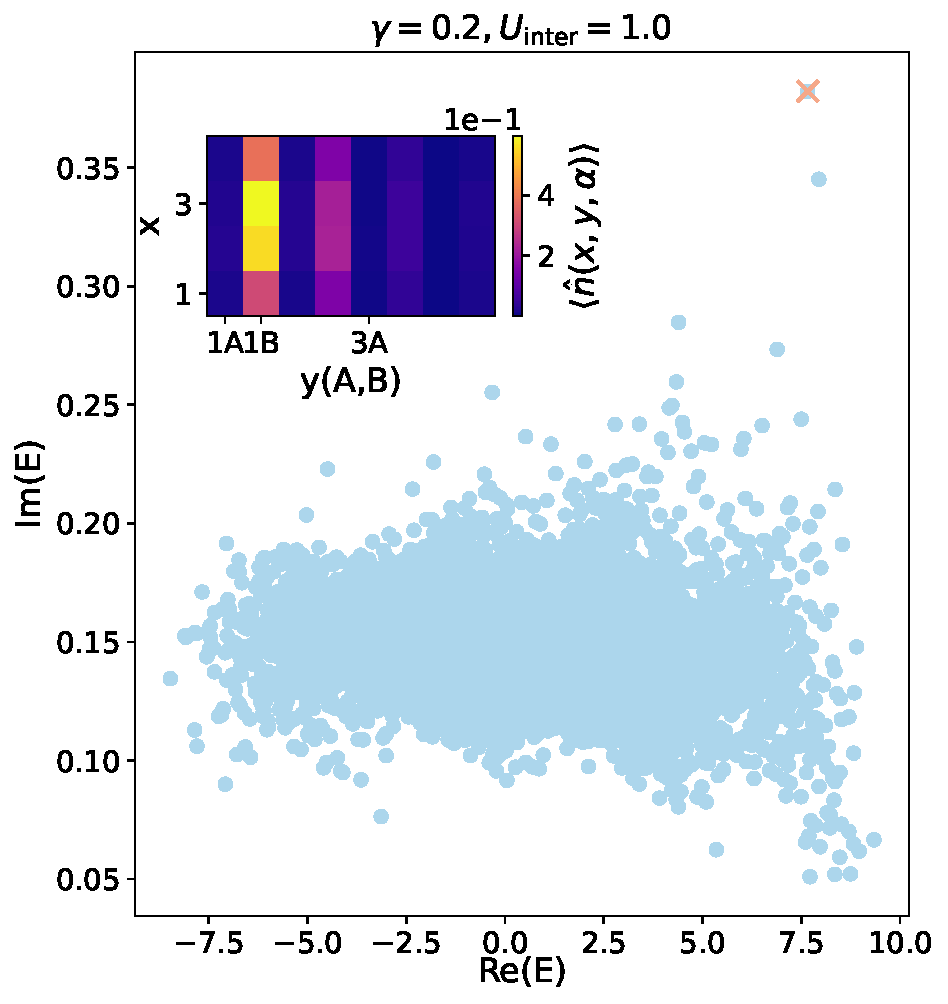
\includegraphics[width=0.47\linewidth]{picture2/ThreeExitation_L4_Spectrum.pdf}
			\begin{overpic}[width=0.47\linewidth]{Picture/ThreeExcitation_Popu_Interaction.pdf}
				% \put(-150,175){(a)}
				\put(-93,98){(a)}
				% \put(-150,98){(b)}
				\put(0,98){(b)}
				% \put(49,54){(d)}
			\end{overpic}
			% \caption{图片1说明}
			% \label{fig:img1}
		\end{minipage}
		% \caption{图片4说明}
		% \label{fig:img4}
		\caption{
			(a) The spectrum and average particle number per lattice site in the three-excitation subspace. The non-Hermitian gain ($\gamma=0.2$) is applied to unit cells at the $y=1$ boundary, and the many-body interaction is $\hat{H}_{\text{inter}}$. The system size is $L_x=L_y=4$. The onsite potential is $u=-1.5$.
		(b) The parameters $\mathcal{P}_{x,y,\alpha}$ at time $t=20$ and $t=60$ under different interaction strengths. Gain is applied to the $y=1$ unit cell. The system size is $L_x=L_y=4$, and the onsite potential is $u=-1.5$. The number of randomly selected initial quantum states is $N_{\text{samp}}=10^4$. 
		}
		\label{fig:03_Supple}
	\end{figure*}


	% Due to the commutation between the number operator and the Hamiltonian, excitation subspaces are decoupled. 
	We have shown that the hybrid chiral skin correlated states in the three-excitation subspace for system size $L_x = L_y =5$ before.
	%In Fig.\ref{fig:03} (a), we present the energy spectrum, the eigenstate with the largest imaginary eigenvalue, and the average particle number of this eigenstate for the non-Hermitian Hamiltonian and the non-Hermitian many-body Hamiltonian. The complex energy of this eigenstate is marked with an orange cross in the spectrum. 
	The basis in the three-excitation subspace are
	% $\{\ket{11100\cdots}, \ket{11010\cdots}, \ket{10110\cdots},\cdots\}$, 
	\begin{equation}
		\begin{split}
		\{\ket{(11)_{1,1}(10)_{1,2}(00)_{1,3}\cdots}, \ket{(11)_{1,1}(01)_{1,2}(00)_{1,3}\cdots}, \\
		\ket{(10)_{1,1}(11)_{1,2}(00)_{1,3}\cdots},\cdots\}, 
		\end{split}
	\end{equation}
	which represent all possible configurations of three fermions in the system. 
    These basis vectors are arranged in descending order according to the binary representation, which corresponds to the basis states. For example, basis $\ket{(11)_{1,1}(10)_{1,2}(00)_{1,3}\cdots}$ is labelled as basis 1, and basis $\ket{(10)_{1,1}(11)_{1,2}(00)_{1,3}\cdots}$ is labeled as basis 2. 
	We also perform numerical diagonalization of the non-Hermitian many-body Hamiltonian with the Arnorldi method~\cite{arnoldi1951principle} for system size $L_x = L_y = 8$ in the three-excitation subspace. Our results demonstrate the persistence of hybrid chiral skin correlated states in higher excitation subspaces (Fig.~\ref{fig:03} (a)).
	For the inter-cell interaction case, the three-particle correlation function reveals strong spatial correlation between the locations of three particles. Particles preferentially occupy adjacent sites ($\Delta x =1$) along $y=1$. The particles are also more localized on the sublattice $B$. 

	
	The mechanism of generating the hybrid chiral skin correlated states can be analyzed with the Fock state representation. 
	We focus on the states with the three particles located at the positions $(x,y)=(1,1), (1,2)$, $(2,1)$ and $(3,1)$ (Fig.~\ref{fig:03} (b)).
	%We consider a system with four unit cells and three particles under many-body interaction $\hat{H}_{\text{inter}}$ (Fig.~\ref{fig:03_Supple} (b)). 
	In Fig.~\ref{fig:03} (b), blue wavy lines denote non-Hermitian pumping, which is restricted to the first three unit cells, while black arrows indicate the hopping term in $\hat{H}_{\text{QWZ}}$. The number of blue wavy lines indicates the magnitude of the non-Hermitian pumping effect.
	% A particle at $B$ sublattice of the unit cell is denoted as $\ket{\uparrow}$, and a particle at $A$ sublattice of the unit cell is denoted as $\ket{\downarrow}$. When $u<0$, the particle at $B$ sublattice has a higher energy. % 在双激发介绍过了。
	For the two-dimensional system, gain is applied to the unit cells along the boundary at $y=1$.
	In the evolution of the non-Hermitian part, particles are predominantly pumped into unit cells with gain. The interaction-induced energy gap suppresses the transition from the state 
	% $\ket{\uparrow\uparrow\uparrow0}$ to $\ket{\uparrow\uparrow0\uparrow}$,
	$\ket{(01)_{1,1}(01)_{2,1}(01)_{3,1}\cdots(00)_{1,2}\cdots}$ to $\ket{(00)_{1,1}(01)_{2,1}(01)_{3,1}\cdots(01)_{1,2}\cdots}$,
	 thereby preventing further transitions out of the unit cells with gain. 
	Conversely, state $\ket{(11)_{1,1}(01)_{2,1}(00)_{3,1}\cdots(00)_{1,2}\cdots}$ can transition to the state $\ket{(10)_{1,1}(01)_{2,1}(00)_{3,1}\cdots(01)_{1,2}\cdots}$ 
	without energy difference, allowing particles to transition out of the unit cells with gain. This transition stems from the absence of energy differences between these two states, as shown in Fig.~\ref{fig:03} (b). 
	Moreover, the two-dimensional configuration enables direct transitions from the first three unit cells to the unit cells without gain.
	Through this mechanism, all states in the third row of Fig.~\ref{fig:03} (b) can jump to the state 
	% $\ket{0\uparrow\downarrow\uparrow}$ 
	$\ket{(10)_{1,1}(01)_{2,1}(00)_{3,1}\cdots(01)_{i,2}\cdots}$ ($i=1,2,3$) 
	through two transitions, thereby jumping to the unit cells without gain. 
	The absence of energy difference in these two transitions facilitates efficient particle redistribution.
	% There is no energy difference in these two steps. 
	%Particles will accumulate at the energy level $\ket{(01)_{1,1}(01)_{2,1}(01)_{3,1}\cdots(00)_{1,2}\cdots}$ under time evolution of non-Hermitian many-body Hamiltonian. 
	When considering all interactions, particles at the energy level $\ket{(01)_{1,1}(01)_{2,1}(01)_{3,1}\cdots(00)_{1,2}\cdots}$ will be confined under time evolution.
	We observe that even in the three-particle excitation subspace, hybrid chiral skin correlated states exist and are localized at the $B$ sublattice. 

	In system size $L_x = L_y = 4$, we investigate the evolution of the system starting from any three-particle excited state at times $t = 20$ and $t = 60$, respectively. 
	At this point, we choose the system size $L_x=L_y=4$, whose spectrum is shown in Fig.~\ref{fig:03_Supple} (a). 
	% At this point, we choose the system size $L_x=L_y=4$, whose spectrum is similar to that in Fig.~\ref{fig:03} (a) ($L=9$). 
	% The corresponding spectral details are presented in the Appendix.~\ref{sec:AddtionalSpectrum3}.
	We measure the particle number operator at different lattice sites and record $\mathcal{P}_{x,y,\alpha}$ in Eq.~\eqref{eq:NumbEvent} where the average particle number exceeds $1/(2L_x)$. The results are presented in Fig.~\ref{fig:03_Supple} (b).
	For the Hermitian many-body Hamiltonian, the number of events $\mathcal{P}_{x,y,\alpha}$ decreases as the interaction strength $\vert U_{\text{inter}}\vert $ increases, indicating that the system evolves toward a delocalized state as the interaction strength increases. 
	In contrast, for the non-Hermitian many-body Hamiltonian, the number of events $\mathcal{P}_{1,1,B}$ at site $(1,1,B)$ increases as $\vert U_{\text{inter}}\vert$ increases, while $\mathcal{P}_{1,3,B}$ decreases as $\vert U_{\text{inter}}\vert$ increases. 
	The Hamiltonian with interaction strength $U_{\text{inter}}$ can be mapped to the Hamiltonian with interaction strength $-U_{\text{inter}}$ under the $\mathcal{PT}$ transformation.
	%, as shown in Appendix~\ref{sec:symmetry_Hamiltonian}.
	When evolving from a random three-particle excited state, the system exhibits localization signals at the $B$ sites of the gain unit cells at $t=60$.
	In about $100\%$ of the cases, the average particle number exceeds $1/(2L_x)$ at least one site (Fig.~\ref{fig:03_Supple}(b)).

	Here, we have discussed the hybrid chiral skin correlated states in the two and three-excitation subspaces. The many-body interaction induces these strong localized states, which cannot be found in the single-particle non-Hermitian Hamiltonian. This hybrid state can exist in the even more excitation subspaces, and the mechanism is similar to those in the two and three-excitation subspaces. 
	When the gain is applied at $y=1$ boundary, the amplitude of state $\ket{(01)_{1,1}(01)_{2,1}\cdots(01)_{n,1}(00)_{n+1,1}\cdots(00)_{1,2}\cdots}$ is enhanced compared to other states in which particles occupy unit cells without gain ($y\neq 1$), under the evolution of $\hat{H}_{\text{im}}$. Moreover, this state is isolated from lower-energy states by a large gap under the evolution of the Hermitian Hamiltonians, such as $\hat{H}_{\text{QWZ}}$ and $\hat{H}_{\text{inter}}$, while other states are either degenerate or separated by relatively small gaps. The amplitude enhancement and energy gap isolation of $\ket{(01)_{1,1}(01)_{2,1}\cdots(01)_{n,1}(00)_{n+1,1}\cdots(00)_{1,2}\cdots}$ enable the emergence of hybrid chiral skin correlated states in the $n$-excitation subspace. 


	% If in two-column mode, this environment will change to single-column
	% format so that long equations can be displayed. Use
	% sparingly.
	%\begin{widetext}
	% put long equation here
	%\end{widetext}
	
	% figures should be put into the text as floats.
	% Use the graphics or graphicx packages (distributed with LaTeX2e)
	% and the \includegraphics macro defined in those packages.
	% See the LaTeX Graphics Companion by Michel Goosens, Sebastian Rahtz,
	% and Frank Mittelbach for instance.
	%
	% Here is an example of the general form of a figure:
	% Fill in the caption in the braces of the \caption{} command. Put the label
	% that you will use with \ref{} command in the braces of the \label{} command.
	% Use the figure* environment if the figure should span across the
	% entire page. There is no need to do explicit centering.
	
	% \begin{figure}
		% \includegraphics{}%
		% \caption{\label{}}
		% \end{figure}
	
	% Surround figure environment with turnpage environment for landscape
	% figure
	% \begin{turnpage}
		% \begin{figure}
			% \includegraphics{}%
			% \caption{\label{}}
			% \end{figure}
		% \end{turnpage}
	
	% tables should appear as floats within the text
	%
	% Here is an example of the general form of a table:
	% Fill in the caption in the braces of the \caption{} command. Put the label
	% that you will use with \ref{} command in the braces of the \label{} command.
	% Insert the column specifiers (l, r, c, d, etc.) in the empty braces of the
	% \begin{tabular}{} command.
		% The ruledtabular enviroment adds doubled rules to table and sets a
		% reasonable default table settings.
		% Use the table* environment to get a full-width table in two-column
		% Add \usepackage{longtable} and the longtable (or longtable*}
	% environment for nicely formatted long tables. Or use the the [H]
	% placement option to break a long table (with less control than 
	% in longtable).
	% \begin{table}%[H] add [H] placement to break table across pages
		% \caption{\label{}}
		% \begin{ruledtabular}
			% \begin{tabular}{}
				% Lines of table here ending with \\
				% \end{tabular}
			% \end{ruledtabular}
		% \end{table}
	
	% Surround table environment with turnpage environment for landscape
	% table
	% \begin{turnpage}
		% \begin{table}
			% \caption{\label{}}
			% \begin{ruledtabular}
				% \begin{tabular}{}
					% \end{tabular}
				% \end{ruledtabular}
			% \end{table}
		% \end{turnpage}
	
	% Specify following sections are appendices. Use \appendix* if there
	% only one appendix.
	%\appendix
	%\section{}
	
	% If you have acknowledgments, this puts in the proper section head.
	%\begin{acknowledgments}
	% put your acknowledgments here.
	%\end{acknowledgments}
	
	
	
\end{document}
%
% ****** End of file apstemplate.tex ******